\documentclass[a4paper]{jpconf}
\usepackage{amsmath}
\usepackage{amssymb}
\usepackage[UKenglish]{babel}
\usepackage{graphicx}
\usepackage{hyperref}
\hypersetup{colorlinks=false, bookmarks=true}
\usepackage{float}
\usepackage{comment}
\usepackage{caption}
\usepackage[skip=0.5ex]{subcaption}
\usepackage{xcolor}

\hyphenation{few-femto-second}

\begin{document}
%\maketitle

\twocolumn[

\pagenumbering{arabic}
\title{Modelling of nonlinear light up-conversion from intense femtosecond laser pulses}
\author{David Amorim (University of Glasgow)}
\address{DESY Summer Student Programme 2023 \\ Group:  Attosecond Science (CFEL-ATTO) \\ Institute: Centre for Free-Electron Laser Science (CFEL)\\ Supervisor: Josina Hahne}

\begin{abstract}
Ultrashort ultraviolet (UV) laser pulses can be produced via nonlinear optical processes in noble gasses based on few-femtosecond near-infrared (NIR) input pulses. The theoretical modelling of these effects can be challenging, however, as many common pulse propagation equations are based on approximations that do not hold for ultrashort pulses. 
This report presents numerical simulations of UV generations in the femtosecond regime using the propagation solver \textit{Luna.jl}. \par 
Despite using a heavily simplified gas distribution model, the simulations could reproduce general trends and qualitative features of experimentally obtained UV spectra and pulse energies. 


 The simulated UV spectra for Argon and Neon agree qualitativelyl with measured data across different pressures and beam powers. The simulations could be used to show that ionisation-induced self-steepening contributes to spectral broadening and pulse compression, in agreement with similar studies in the literature. It was further demonstrated that using chirped NIR input pulses can increase the spectral bandwidth. The simulations also supported experimental data on the improved performance of a new gas chip design. \par 

The simulations presented here serve as a proof of concept that, 
 
REWRITE THIS!!! 
 
 
With further modifications and extensions, the simulations presented here could form the basis of a robust theoretical framework to complement experimental results and aid experimental design.  
\end{abstract}
]


\thispagestyle{plain}
\pagestyle{plain}
\setlength{\footskip}{20pt}

\section{Introduction}
The electronic motion associated with chemical reactions and atomic energy transitions takes place on femotsecond ($1 \text{fs} = 10^{-15} \text{s}$) to attosecond ($1 \text{as} = 10^{-18} \text{s}$) time scales. Time-resolved imaging of molecular dynamics therefore requires ultrashort laser pulses in the few-femtosecond regime. An important type of electronic motion is that excited by the absorption of ultraviolet (UV) radiation: a variety of biochemical processes, such as DNA damage, are known to be caused by UV excitation. Generating few-femtosecond UV pulses for time-resolved measurements of UV-excited molecules plays a crucial part in further understanding and eventually controlling these effects. \par 
The CFEL-ATTO group at DESY produces ultrashort UV pulses in the femtosecond regime via third-harmonic generation (THG) in a gas cell \cite{galli2019}. This process is sensitive to a large range of parameters which affect the duration and energy of the generated UV pulse. Numerical simulations of the interactions between the laser pulse and the gas can therefore be advantageous to better understand how THG takes place and how it is affected by the experimental conditions. The theoretical description of UV generation in the femtosecond regime is challenging, however, since the simplifying assumptions commonly used in pulse propagation calculations do not apply to ultrashort laser pulses. \par 
This report summarises the work carried out as part of a DESY Summer Student project focussed on producing simulations of the THG process for few-femtosecond pulses. The simulations were mainly carried out using the propagation solver \textit{Luna.jl} (\cite{brahms2023}). The aim of the simulations was to reproduce the experimental conditions in the gas, in order to study which effects dominate the THG process and the shaping of the UV pulse. \par 
ADD PROOF OF CONCEPT DISCLAIMER??

\section{Background}
This section gives a brief overview of key properties of ultrashort laser pulses,  THG and other relevant nonlinear optical effects, as well as the differential equation describing the propagation of ultrafast laser pulses. An in-depth treatment of these topics can be found in textbooks like \cite{keller2021, new2011}. \par 
The final subsection then presents the experimental conditions of UV generation, which the simulations aim to replicate. 

\subsection{Ultrashort Laser Pulses}
An ultrashort laser pulse can be described as a carrier wave at carrier frequency $\omega_0$ with an amplitude modulated by an envelope function. In the femtosecond domain the envelope may only contain a few cycles of the carrier wave. Using the analytic representation of the electric field vector the time-domain representation of an ultrashort laser pulse can be written as 
\begin{equation}
\mathbf{E}(t, \mathbf{r}) = \mathbf{A}(t, \mathbf{r}) e^{i[ \omega_o t + \phi(t)]},
\end{equation}
where $\mathbf{A}(t, \mathbf{r})$ represents the envelope function and $\phi(t)$ is the temporal phase. The vectorial nature of the envelope takes into account the polarisation of the pulse. Similarly, the frequency-domain representation is 
\begin{equation}
\mathbf{E}(\omega, \mathbf{r}) = \mathbf{A}'(\omega, \mathbf{r}) e^{i \varphi(\omega)},
\end{equation}
where $\varphi(\omega)$ is the spectral phase. Note that the effect of the carrier term in the frequency domain is merely a shift along the frequency axis and can be thus be absorbed in the definition of $\omega$. \par 
The spectral and temporal phase are commonly expanded as Taylor-series, with the symbols $\phi_n \equiv \frac{\partial^n \phi}{\partial t^n}$ and $\varphi_n \equiv \frac{\partial^n \varphi}{\partial \omega^n}$ used to denote the series coefficients. The zeroth-order terms of both expansions are the same, $\phi_0 = \varphi_0$, and correspond to the carrier-envelope phase (CEP), also known as the absolute phase. The CEP desribes the phase difference between the carrier and the envelope and is particularly relevant for few-cycle pulses. A laser pulse with no terms in $\varphi(\omega)$ higher than $\varphi_0$ is said to be transform-limited. A pulse is said to be chirped if there are nonlinear terms in $\phi(t)$ or $\varphi(\omega)$. \par 
The presence of chirp may result in both spectral and temporal broadening of the pulse envelope. A convenient measure of chirp is therefore the so-called time-bandwidth product $\Delta \omega \Delta t$, where $\Delta \omega$ is the full-width half-maximum (FWHM) of $\mathbf{A}'(\omega, \mathbf{r})$ and $\Delta t$ the FWHM of $\mathbf{A}(t, \mathbf{r})$. It can be shown that the time-bandwidth product is minimised for transform-limited, i.e. unchirped, pulses. \par 
The effects on a laser pulse when travelling through a medium are described via additional terms in the spectral phase: $\varphi(\omega) \to \varphi(\omega) + [\beta(\omega) + i \alpha(\omega)]L$, where $L$ corresponds to the distance travelled in a medium, $\beta(\omega)$ is the propagation coefficient, and $\alpha(\omega)$ the absorption coefficient. The latter term represents an attenuation of the pulse while the former has the effect of introducing chirp (provided the Taylor-expansion of $\beta(\omega)$ has non-zero terms higher than $\beta_1$). Note that depending on the signs of the quantities involved, the chirp due to $\beta(\omega)$ will either increase or compensate the existing chirp on the pulse. Thus, an initially positively chirped pulse will further broaden upon propagation through a normally dispersive medium while a negatively chirped pulse will be compressed. The opposite effect is observed in anomalously dispersive media. The coefficient $\beta_2$ in the Taylor-expansion of $\beta(\omega)$ is of particular practical importance and generally known as group velcity delay (GVD).

\subsection{Nonlinear Optics and THG}
For most materials, the polarisation response to an electric field of moderate intensity is linear. The peak intensities reached in ultrashort laser pulses are large enough, however, for this approximation to become invalid and nonlinear polarisation components to appear. The resulting polarisation can then be represented as a combination of a linear and a nonlinear term: $\mathbf{P}(t, \mathbf{r}) = \mathbf{P}^\text{L}(t, \mathbf{r}) + \mathbf{P}^\text{NL}(t, \mathbf{r})$. \par 
The linear polarisation is given by the familiar expression $\mathbf{P}^\text{L}(t, \mathbf{r}) = \epsilon_0 \chi_e \mathbf{E}(t, \mathbf{r})$, where $\chi_e$ is the (linear) electric susceptibility. The nonlinear term, $\mathbf{P}^\text{NL}(t, \mathbf{r})$, on the other hand, is less trivial. It can be approximated using a perturbative approach in combination with a term that takes into account the effects of photoionisation, which is non-perturbative:
\begin{equation}\label{eq:p_nl}
\mathbf{P}^\text{NL}(t, \mathbf{r}) = \epsilon_0 \sum_{n=2} \chi^{(n)} [\mathbf{E}(t, \mathbf{r})]^n + \mathbf{P}^\text{ion}(t, \mathbf{r}),
\end{equation}
where $\chi^{(n)}$ is the $n$-th order electric susceptibility. Note that for gases the assumption that the higher-order susceptibilities are frequency-independent scalars is a good approximation. Further note that the series expansion starts at the quadratic term as the linear term is contained in $\mathbf{P}^\text{L}(t, \mathbf{r})$.  \par 
In centrosymmetric media such as gases all even-order susceptibilities necessarily vanish, so that the dominant term in the expansion is the third-order term. Higher-order contributions can be neglected to a good approximation, so that \eqref{eq:p_nl} reduces to
\begin{equation}\label{eq:p_nl_simpl}
\mathbf{P}^\text{NL}(t, \mathbf{r}) = \epsilon_0 \chi^{(3)} [\mathbf{E}(t, \mathbf{r})]^3 + \mathbf{P}^\text{ion}(t, \mathbf{r}),
\end{equation}
where $[\mathbf{E}(t, \mathbf{r})]^3 \equiv \mathbf{E}(t, \mathbf{r}) |\mathbf{E}(t, \mathbf{r})|^2$. 
The first term in \eqref{eq:p_nl_simpl} is known as the Kerr term and its presence leads directly to THG. This can be seen when considering an oscillating electric field $\mathbf{E}(t, \mathbf{r}) = \hat{\mathbf{E}}(t, \mathbf{r})\cos(\omega t)$: the resulting Kerr response then is 
\begin{align}\label{eq:Kerr_response}
\nonumber  \mathbf{P}^\text{Kerr}(t,\mathbf{r}) &= \epsilon_0 \chi^{(3)} [\hat{\mathbf{E}}(t, \mathbf{r})]^3 \cos^3(\omega t) \\ &= \frac{\epsilon_0}{4}  \chi^{(3)} [\hat{\mathbf{E}}(t, \mathbf{r})]^3 \left\{ \cos (3\omega t) +  3 \cos(\omega t)\right\}.
\end{align}
The first summand in \eqref{eq:Kerr_response} corresponds to a field contribution oscillating at the frequency $3 \omega$. Thus, a pump wave at the fundamental frequency $\omega$ will generate a co-propagating frequency-tripled field. This process can be identified as THG. Note that THG is just once instance of a range of nonlinear optical effects which result in the generation of higher-frequency waves from a driving field, generally known as frequency up-conversion. \par 
The intensity of the third harmonic is determined by the value of $\chi^{(3)}$ in a given medium as well as by the intensity of the driving field. This also implies that, since the intensity of the fundamental pulse is highest at the peak of the envelope, THG conversion is more efficient there than at the edges of the pulse, so that the third harmonic pulse is narrower in time than the input pulse by a factor of $\sim\sqrt{3}$. \par 
 A further effect to consider is that the third harmonic is generated in phase with the driving wave at each point in the nonlinear medium. Thus, in dispersive media there will be phase differences between third harmonic contributions generated at different points along the medium. This can result in destructive interference and thus lower the THG conversion efficiency. \par 
The second summand in \eqref{eq:Kerr_response}, corresponding to polarisation response at the fundamental frequency, is also significant: its effect is a correction term in the refractive index that is proportional to the intensity of the driving field. This intensity-dependent refractive index (IDRI) produced by the Kerr term has important implications for the propagation of laser pulses in nonlinear media. These include self-steepening, which describes the effect of the peak of the pulse experiencing a different group velocity in a dispersive medium than the wings. This results in the leading edge of the pulse or, in the case of anomalous dispersion, the trailing edge, to get steeper on propagation, corresponding to temporal compression and spectral broadening. \par 
After having considered the effects of the Kerr term in the previous paragraphs, we now turn to the second term in \eqref{eq:p_nl}: the nonlinear polarisation due to photoionisation. The highly energetic driving pulse can ionise the atoms or molecules in the nonlinear medium, resulting in the presence of free electrons. This has a two-fold effect on pulse propagation and THG. On the one hand, the pump field is depleted since it must overcome the atomic ionisation potential, so that less energy is available to drive THG. On the other hand, the freed electrons also interact electromagnetically with the fundamental and third harmonic fields, which results in spatio-temporal reshaping of the pulses. Thus, despite ionisation limiting the achievable third harmonic pulse energy, it can aid in further shortening the generated pulses. \par 
The theoretical treatment of $\mathbf{P}^\text{ion}(t, \mathbf{r})$ is significantly more sophisticated than that of the Kerr term. As is derived in \cite{geissler1999}:
\begin{equation}\label{eq:p_ion}
\frac{\partial}{\partial t} \mathbf{P}^\text{ion}(t, \mathbf{r}) = \frac{I_p}{\mathbf{E}(t)} \frac{\partial n_e}{\partial t} + \frac{e^2}{m_e^2} \int_{-\infty}^t n_e(t') \mathbf{E}(t')dt',
\end{equation} 
where $n_e(t)$ is the number of free electrons at any point in time, $I_p$ is the ionisation potential, and $e$, $m_e$ represent the electron charge and mass, respectively. The value of $n_e(t)$ can be found from 
\begin{equation}
\frac{\partial n_e}{\partial t} = (n_e - n_0) W(\mathbf{E}),
\end{equation}
where $n_0$ is the initial number of neutral atoms and $W(\mathbf{E})$ is the ionisation rate, which can be calculated from the so-called PPT model of tunnel ionisation. 

\subsection{The Unidirectional Pulse Propagation Equation}

A variety of different differential equations  can be used to describe the propagation of laser pulses. Many of them are derived under the slowly-varying- envelope assumption (SVEA), which approximates the carrier wave to change significantly more quickly in space and time than the pulse envelope. The SVEA does not hold for ultrashort pulses, however, and hence many commonly used pulse propagation equations are not suitable for the study of few-femtosecond pulses. The unidirectional pulse propagation equation (UPPE) is derived directly from Maxwell's equations without additional approximations, see \cite{kolesik2004}, and therefore can be applied to ultrashort pulses. It is the differential equation used by \textit{Luna.jl} to simulate laser pulse propagation. This section gives a brief overview of the UPPE and how it is solved in \textit{Luna.jl}. For more details on numerical solutions of the UPPE see the \textit{Luna.jl} documentation, \cite{brahms2023}, as well as \cite{tani2014}. \par 
The general form of the UPPE for a laser pulse of frequency $\omega$ travelling in the $z$-direction is
\begin{align}\label{eq:UPPE}
\nonumber \frac{\partial}{\partial z} \mathbf{E}(\omega, \mathbf{k}_\perp, z)&= \mathcal{L}(\omega, z)\mathbf{E}(\omega, \mathbf{k}_\perp, z) \\ &+ \frac{i \omega}{N} \mathbf{P}^\text{NL}(\omega, \mathbf{k}_\perp, z),
\end{align}
where $\mathbf{E}(\omega, \mathbf{k}_\perp, z)$ is the reciprocal-space electric field amplitude in the frequency domain, $\mathbf{k}_\perp$ is the transverse spatial frequency vector,  $\mathcal{L}(\omega, z)$ is a linear operator describing dispersion and absorption, $\mathbf{P}^\text{NL}(\omega, \mathbf{k}_\perp, z)$ is the frequency-domain nonlinear polarisation in reciprocal space and $N$ is a normalisation factor. \par 
For a laser pulse propagating in a gas, not confined by a fibre or waveguide, the linear operator $\mathcal{L}(\omega, z)$ is given by 
\begin{equation}\label{eq:Lj}
\mathcal{L}(\omega, z) = i \left( \beta(\omega, z) - \frac{\omega}{v} \right) - \frac{1}{2} \alpha (\omega,z),
\end{equation}
where $\beta(\omega,z)$ is the propagation coefficient of the gas, $v$ is a reference frame velocity (chosen to be the group velocity at the central wavelength $\lambda_0$), and $\alpha(\omega,z)$ is the absorption coefficient of the gas. \par 
As is seen in \eqref{eq:p_nl_simpl} and \eqref{eq:p_ion}, the nonlinear polarisation is naturally calculated from the electric field in real space and the time domain. Thus, numerically solving the UPPE, which is defined in reciprocal space and the frequency domain, requires a cycle of temporal Fourier transforms into and out of the frequency domain as well as transverse spatial transforms into and out reciprocal space at each step. The choice of transverse spatial transform is determined by the geometry of the system. \par 
Since the beam and the channel it propagates through for UV generation are approximately radially symmetric, a zeroth-order Hankel transform is chosen as the transverse spatial transform. This is mathematically equivalent to a  transverse spatial Fourier transform in Cartesian coordinates but is computationally more efficient, as the Hankel transform exploits the symmetry and only involves integration in the radial direction, whereas the transverse spatial Fourier transform is two-dimensional. 
 
\subsection{Experimental Conditions}\label{sec:exp_cond} 
\begin{figure}[h]
\centering
 \begin{subfigure}{0.5\textwidth}
        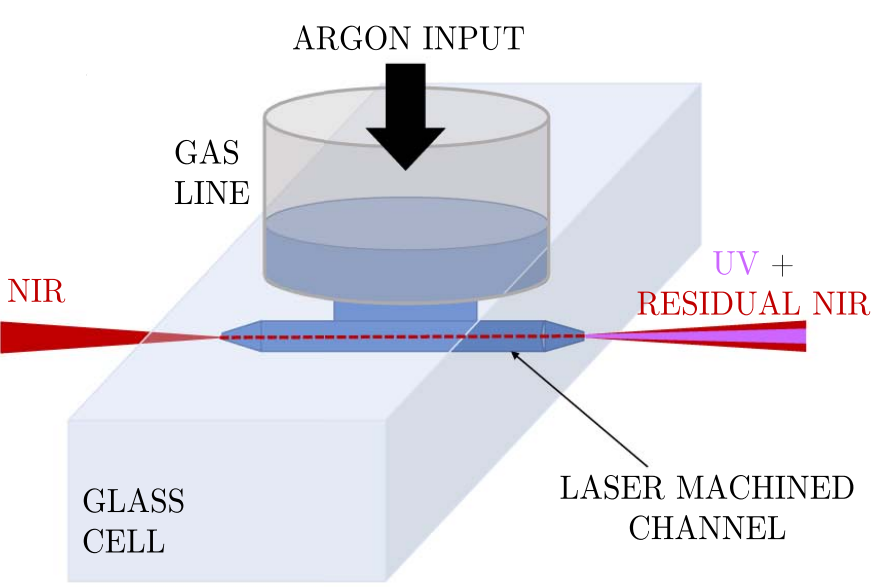
\includegraphics[width=\textwidth]{im/schematic_galli}
   \caption{}\label{im:thg_schematic}
    \end{subfigure}  
 \begin{subfigure}{0.5\textwidth}
        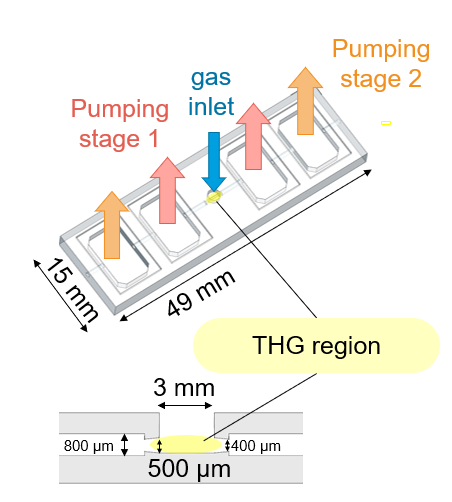
\includegraphics[width=\textwidth]{im/new_chip_edited}
    \caption{}\label{im:new_chip}
    \end{subfigure}
\caption{The fused silica chip used to confine the gas for THG. 
Figure \ref{im:thg_schematic}, reproduced from \cite{galli2019}, shows a simplified schematic of the THG process taking place in the glass cell, without the pumping system, while Figure \ref{im:new_chip}, reproduced from Josina Hahne's master's thesis defence, gives a detailed overview of the chip's design.}
\end{figure}
The CFEL-ATTO group generates few-femtosecond UV laser pulses via THG in a gas cell. This is driven by a pulsed near-infrared (NIR) Ti:sapphire laser with a central wavelength of 800nm and a repetition rate of 1kHz. Various fibre-based pulse-shaping and compression techniques are used to produce NIR pulses with a duration of around 5fs and a pulse energy of up to 3mJ. A fraction of the NIR beam is then linearly polarised and focussed into a vacuum chamber for UV generation, resulting in a spatially approximately Gaussian beam with a beam waist of 65$\mu$m at the focus. The chamber contains a glass chip made of fused silica (SiO$_2$), a gas inlet and a pumping system. Its specifications are central to the THG process and are described in more detail in the following. \par 
The fused silica chip is equipped with a laser machined central 3mm-long channel with a 0.5mm diameter. Pressurised gas, normally Argon or Neon, is pumped through the channel, with a two-stage differential pumping system on both sides of the central interaction region ensuring a tight confinement of the gas in this region. As the pump beam passes through the cell and interacts with the pressurised gas THG takes place, which results in UV pulses being generated. The UV components are then separated from the pump beam upon exiting the vacuum chamber using dispersive mirrors, which reflect in the UV but transmit in the NIR. Figure \ref{im:thg_schematic} shows a simplified schematic of this set-up, without the pumping system. The fused silica chip, including the two pumping stages is shown in Figure \ref{im:new_chip}, with the 3mm central interaction region highlighted. \par 
The fused silica chip shown in Figure \ref{im:new_chip} is an improved design on a simpler  cell which was used previously. The old and new cell have the same 3mm central interaction region but in

NOT REALLY 

 the old design pumping took place further from the gas inlet, resulting in a less tight confinement of the gas in the THG region. 
 
 
 Experimental results demonstrate that the new chip outperforms the old when it comes to UV energies and pulse durations. How this can be related to the difference in gas distribution between the two designs will be explored later. Note that all measurements presented in this report were taken with the new chip in place. 


\section{Simulation Results}

In order to reproduce the experimental conditions described in Section \ref{sec:exp_cond} as closely as possible in the simulations the simulation input was based on measured data, wherever possible. Thus, the time-frequency information as well as the central wavelength of the NIR input pulse used to model the pump beam in the simulations were read in from experimental data. Spatially, the input beam was assumed to be a Gaussian with a beam waist and focus position corresponding to the values used experimentally. \par 
Apart from the profile of the NIR input beam, the most important THG condition to be modelled was the gas density distribution in the fused silica chip. A fully realistic model of the gas distribution, taking into account the geometry of the chip as well as the effects of the differential pumping system, is challenging to obtain. Some efforts to achieve this have been made using the \textit{COMSOL Multiphysics} software but no sufficiently accurate model of the gas distribution throughout the entire chip could be produced at this point. Therefore, the THG simulations focused exclusively on the 3mm central interaction region of the chip. The density distribution in this region was modelled using a gradient based on the central pressure at the gas inlet and the pressure at the edges of the central interaction region, which has been measured to be around 1mbar. The gradient model is based on an interpolation of pressure values between the central and the edge pressure using the equation 
\begin{equation}
p(z)^2 = p(z_0)^2 + (z-z_0) \frac{p(z_1)^2 - p(z_0)^2}{z_1 - z_0}, 
\end{equation}
where $z$ is a point on the between $z_0$ and $z_1$, which are two points at which the pressure is known, such as the centre and edges of the THG region. The density distribution is then inferred from the interpolated pressure distribution. \par 
\begin{figure}[h]
\centering
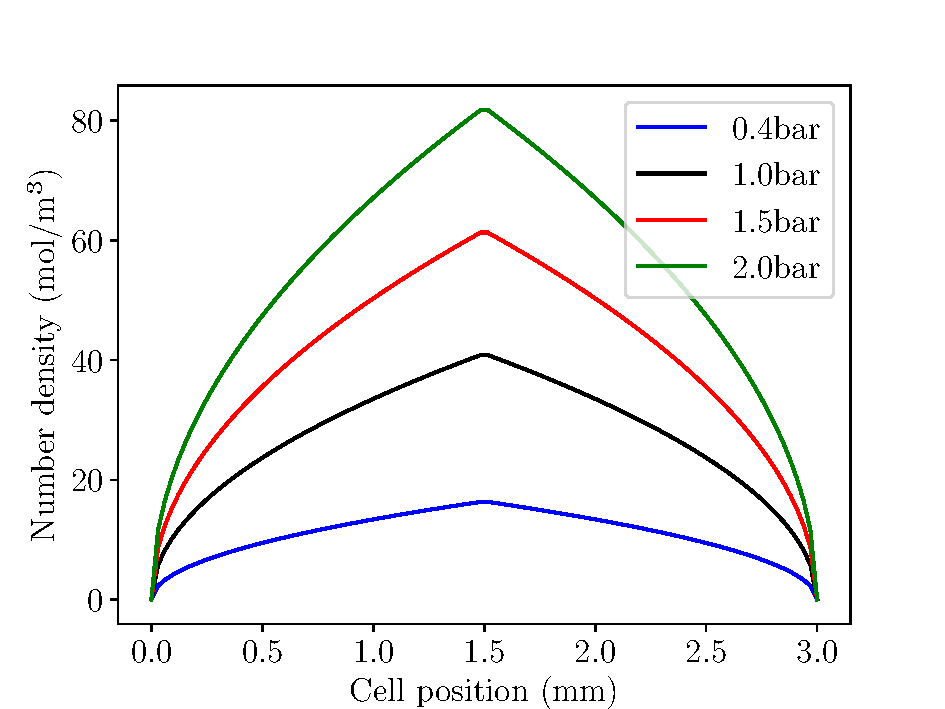
\includegraphics[width=0.5\textwidth]{im/grad_model}
\caption{XXX}\label{im:grad}
\end{figure} 
While discrepancies between this simplified density model and the real distribution are to be expected, especially due the lower-density regions just outside the cell, in which relevant pulse-shaping and absorption processes likely take place, being ignored, the gradient model of the central interaction region can be expected to at least provide qualitatively meaningful results. \par 
In Section XX, the simulations are extended outside the central interaction region in order to compare the performance of the new chip with that of the old cell. The density distributions used in these cases are based on \textit{COMSOL Multiphysics} simulations of the gas flow. As mentioned above, these simulations are only approximate at the present stage, as they do not sufficiently take into account the interactions between gas molecules in the high pressure regions. Thus, the comparison between the cells is a qualitative one. Note that both the old and the new cell are modelled equally well by the gradient model. \par 
While the simulations can be run for a variety of different gases, central pressures and input beam powers, the results presented in this report will, for simplicity, mostly focus on Argon at 150mW NIR power and Neon at 400mW NIR power, with central gas pressures of 0.4bar and 2.0bar, respectively. These values were chosen due to the availability of high quality experimental data at these parameters. 

\subsection{Comparison with Experiment}
This section compares some of the simulation output with experimental data. \par 
\begin{figure}[h]
\centering
 \begin{subfigure}{0.5\textwidth}
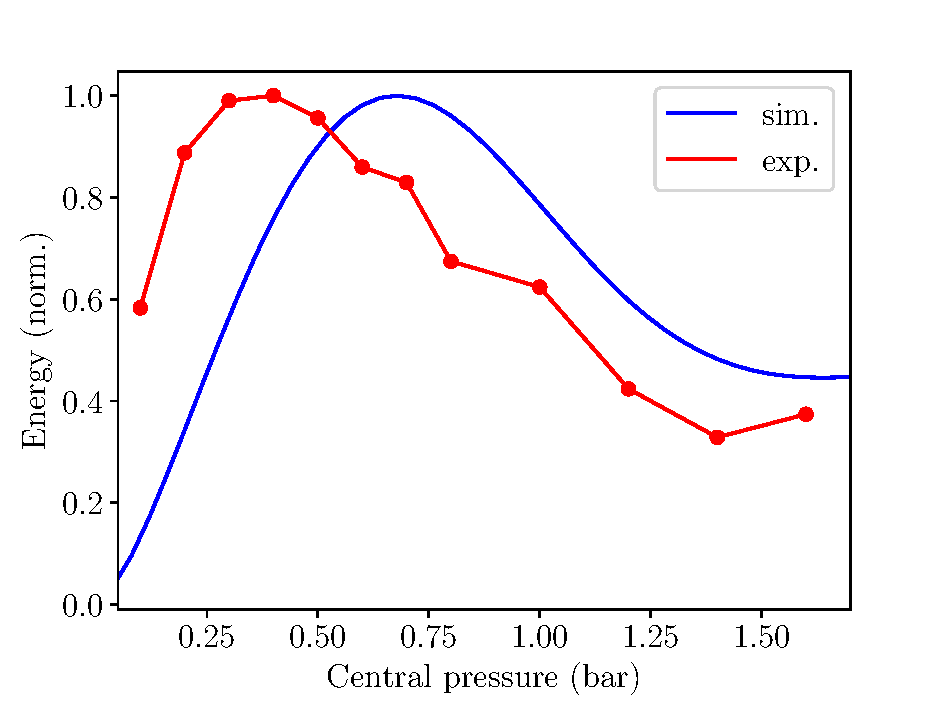
\includegraphics[width=\textwidth]{im/energies_Ar}
\caption{Argon at 150mW NIR beam power}\label{im:sim_v_measured_Ar}
\end{subfigure}
 \begin{subfigure}{0.5\textwidth}
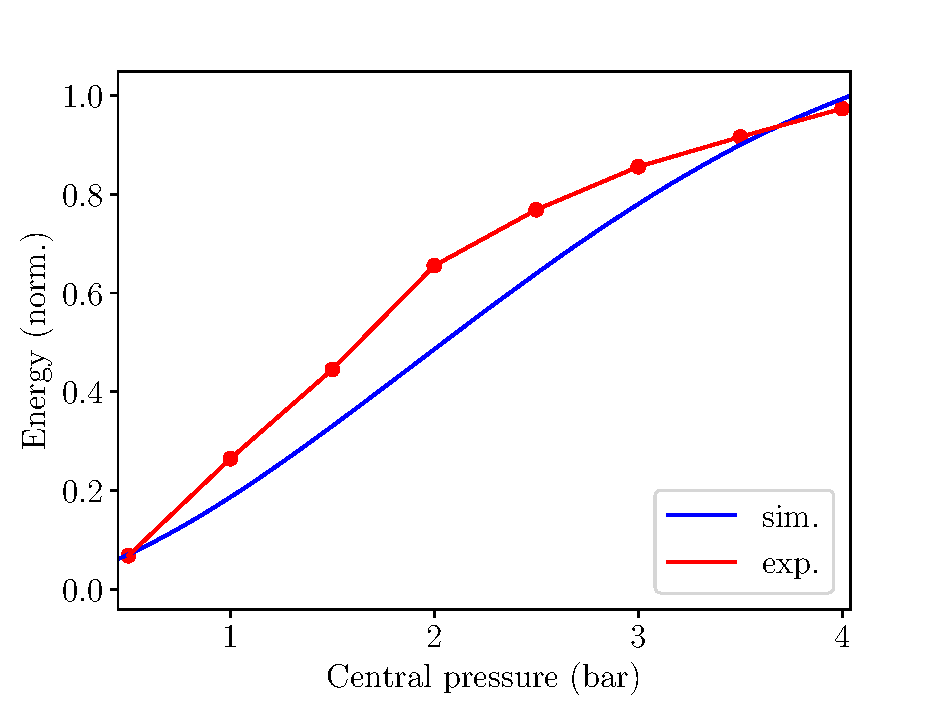
\includegraphics[width=\textwidth]{im/energies_Ne}
\caption{Neon at 400mW NIR beam power}\label{im:sim_v_measured_Ne}
\end{subfigure}
\caption{Simulated and experimental values for UV output energies at different central pressures. Note that the pressure axes of the simulated data have been rescaled and the energy axes normalised.}\label{im:sim_v_measured}
\end{figure}
As can be seen in Figure \ref{im:sim_v_measured}, there is good qualitative agreement between the simulated and measured UV output pulse energies for both Argon and Neon. The energy axes for both plots are normalised to allow for a better qualitative comparison despite a discrepancy between the simulated and measured energies by a factor of roughly ten. This overestimation of the UV energies in the simulation can likely be attributed to the simplistic gas density distribution used, which, for example, does not take into account UV absorption in the low-density regions outside the cell. Similarly, the pressure values for the simulated data had to be rescaled by a factor of 2.5 in both cases to compensate for a mismatch between measured and simulated pressures. The origin of this mismatch, apart from the shortcomings of the gradient model, is the experimental challenge associated with finding an absolute pressure value at the gas inlet, which is why therefore usually approximated with the pressure at the gas pump (???). Taking into account these factors, however, the simulations can clearly reproduce general trends concerning the relationship between UV energies and cell pressure, despite using the simplified gradient model. \par 
Figure \ref{im:sim_v_measured} shows that in both simulations and experiment, UV energies rise with increasing central pressure. This is due to higher pressures being associated with higher gas densities in the cell and hence more polarisable gas atoms, increasing the nonlinear polarisation response and hence the effective value of $\chi^{(3)}$. At higher pressures, the trend slows down and eventually reverses because of ionisation effects: the UV beam in the gas cell becomes sufficiently intense to contribute to ionisation of the gas atoms, resulting in a depleted output beam. Saturation sets in more quickly for Argon than for Neon due to its ionisation potential being lower and its $\chi^{(3)}$ value being higher. \par 
\begin{figure}[h]
\centering
 \begin{subfigure}{0.5\textwidth}
\includegraphics[width=\textwidth]{im/spec_comp_Ar_150mw_2.5scale_0.4bar}
\caption{Argon at 150mW and 0.4bar}\label{im:spec_Ar}
\end{subfigure}
 \begin{subfigure}{0.5\textwidth}
\includegraphics[width=\textwidth]{im/spec_comp_Ne_400mw_2.5scale_2.0bar}
\caption{Neon at 400mW and 2.0bar}\label{im:spec_Ne}
\end{subfigure}
\caption{Simulated and measured UV output spectra. The power values in the subfigure captions refer to the NIR beam power and the pressure values to the central cell pressures. Note that the pressures of the simulated spectra have been rescaled.}\label{im:spec}
\end{figure}
Beyond the UV energies, it is also instructive to consider the simulated UV output spectra. Figure \ref{im:spec} compares the measured and simulated spectra for both Argon and Neon. Despite the shortcomings of the gradient model, the spectra are in fairly good agreement, with the general features of the experimental spectra reproduced in the simulations. As expected, the spectra are centred on roughly 266nm, corresponding to the third harmonic of the central wavelength (800nm) of the NIR input beam. A comparison of simulated and experimental UV spectra across different central pressures is shown in Figure \ref{im:spec_2d}. The simulations clearly reproduce the general trend of higher pressures resulting in a gradual red-shift. Some discrepancies between simulated and measured data are also apparent, however, like the simulations predicting the splitting of the central peak for Argon and the saturation of UV intensities in Neon not being reproduced. 
MENTION OFFSET OF ARGON PRESSURES!!!
\begin{figure*}[h]
\centering
 \begin{subfigure}{0.49\textwidth}
        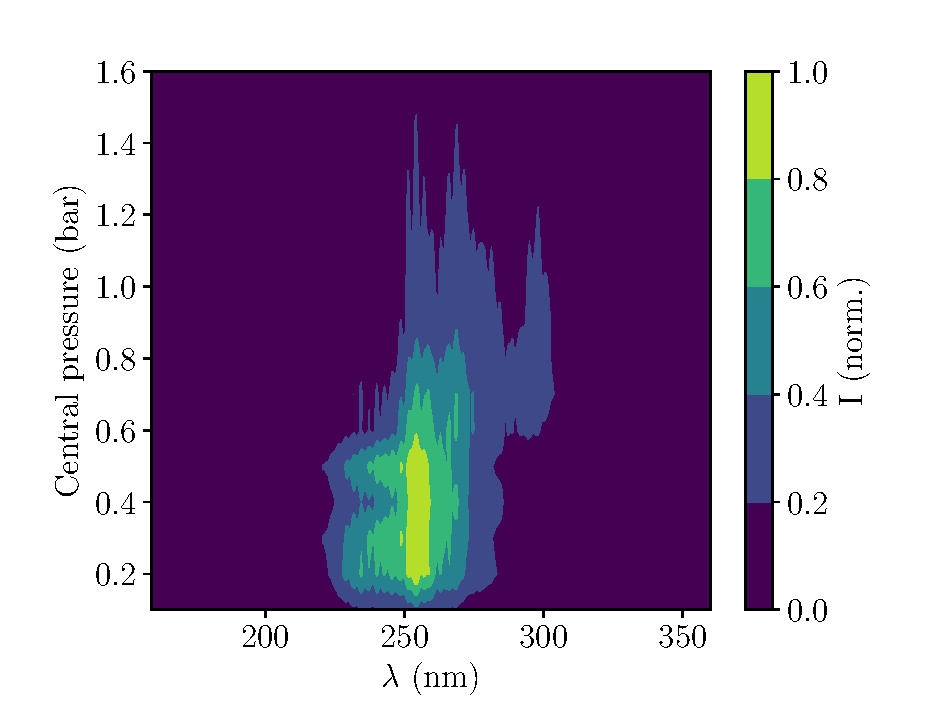
\includegraphics[width=\textwidth]{im/2d_spectra_pres_Ar_150mW_meas}
    \caption{}
    \end{subfigure}
    \begin{subfigure}{0.49\textwidth}
        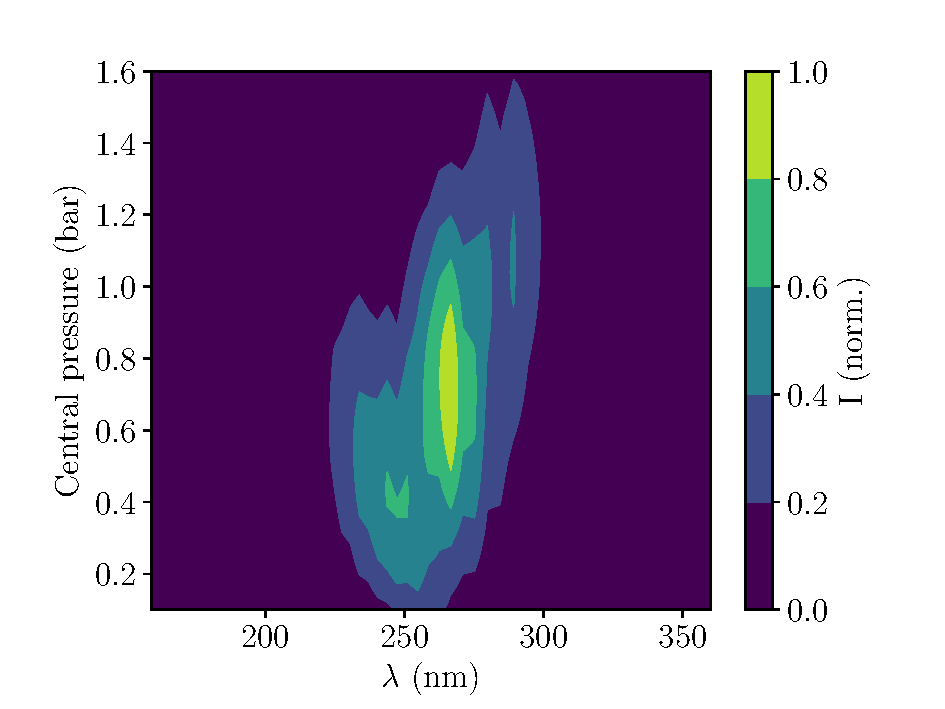
\includegraphics[width=\textwidth]{im/2d_Ar_sim}
    \caption{}
    \end{subfigure}   
     \begin{subfigure}{0.49\textwidth}
        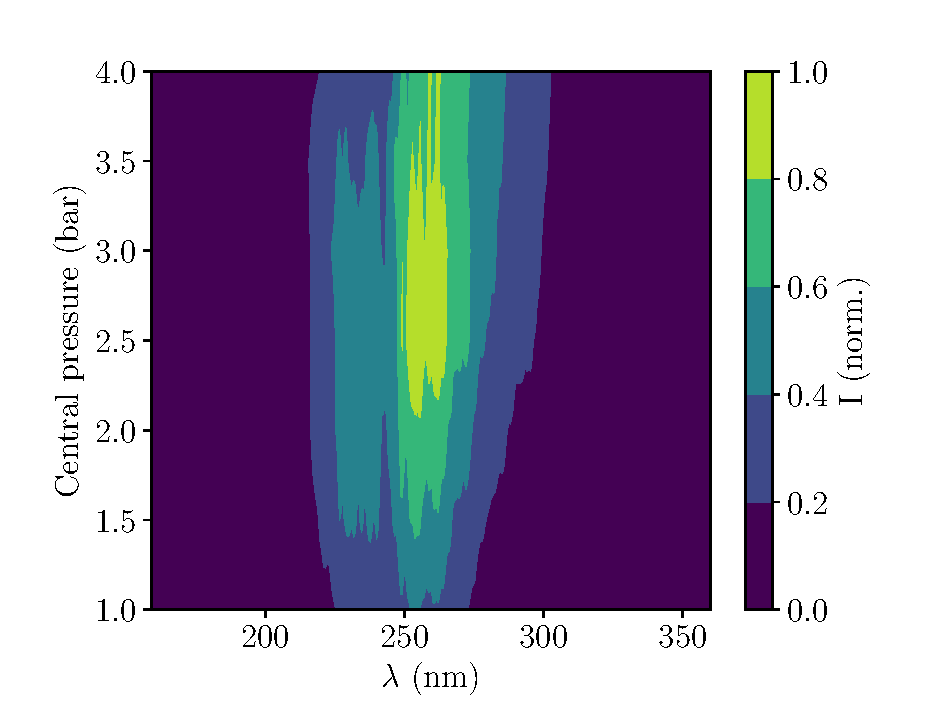
\includegraphics[width=\textwidth]{im/2d_spectra_pres_Ne_400mW_meas}
    \caption{}
    \end{subfigure}
    \begin{subfigure}{0.49\textwidth}
        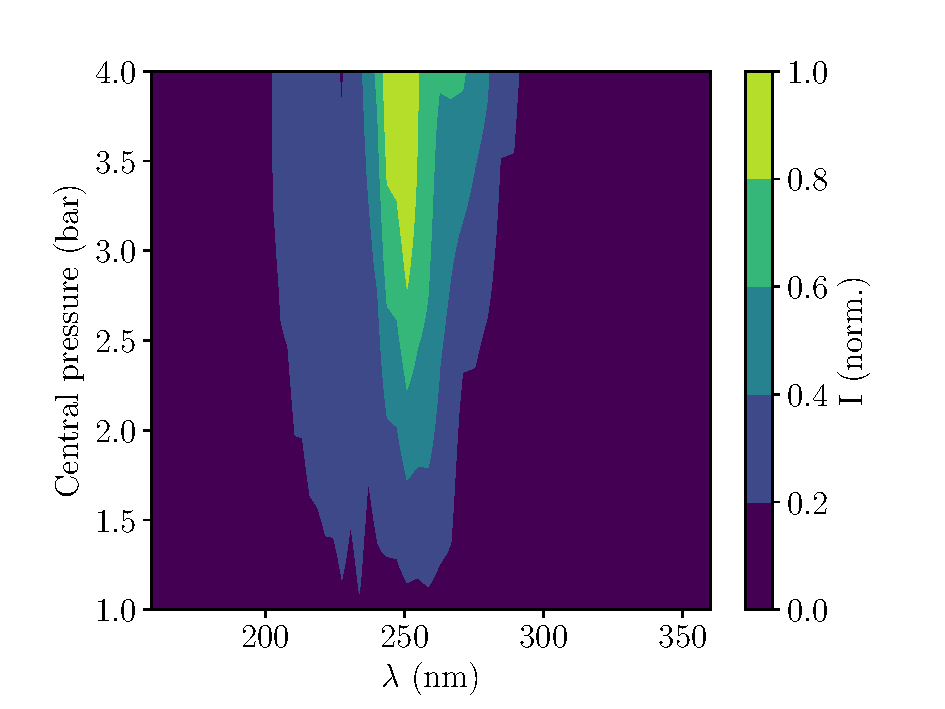
\includegraphics[width=\textwidth]{im/2d_Ne_sim}
    \caption{}
    \end{subfigure}  
\caption{UV output spectra at different central pressures. Measured data is shown in the left column, simulated data with rescaled pressure axes in the right column. The top row corresponds to Argon at 150mW NIR power while the bottom row corresponds to Neon at 400mW NIR power}\label{im:spec_2d}
\end{figure*}
IN THE FOLLOWING: ALWAYS REFER TO RE-SCALED PRESSURE AXES!!

\subsection{Self-steepening and Ionisation}
(REWRITE THIS, ABSOLUTE DRIVEL)
When carrying out UV generation experiments the UV pulses can be analysed with regards to their spectra and energies and to some extend their spatial and temporal profiles can be  resolved. It is not possible to access any of the beam properties within the cell where the pulses are generated, however. Using simulations, a picture of the UV pulses as they are being generated can be obtained which makes accessible some of the effects dominating the THG process. \par 
Note that for concision, only Argon at 150mW NIR power and 0.4bar central pressure is considered here, although equivalent effects can be observed for Neon. 
\par 
One parameter that can be accessed using the simulation is the spatiotemporal beam profile of the UV pulses as they propagate through the central interaction region of the chip. Figure \ref{im:prop} shows how the UV pulses are increasingly deformed and leading-edge self-steepening sets in with increasing propagation distance. 
\begin{figure}[h]
\centering
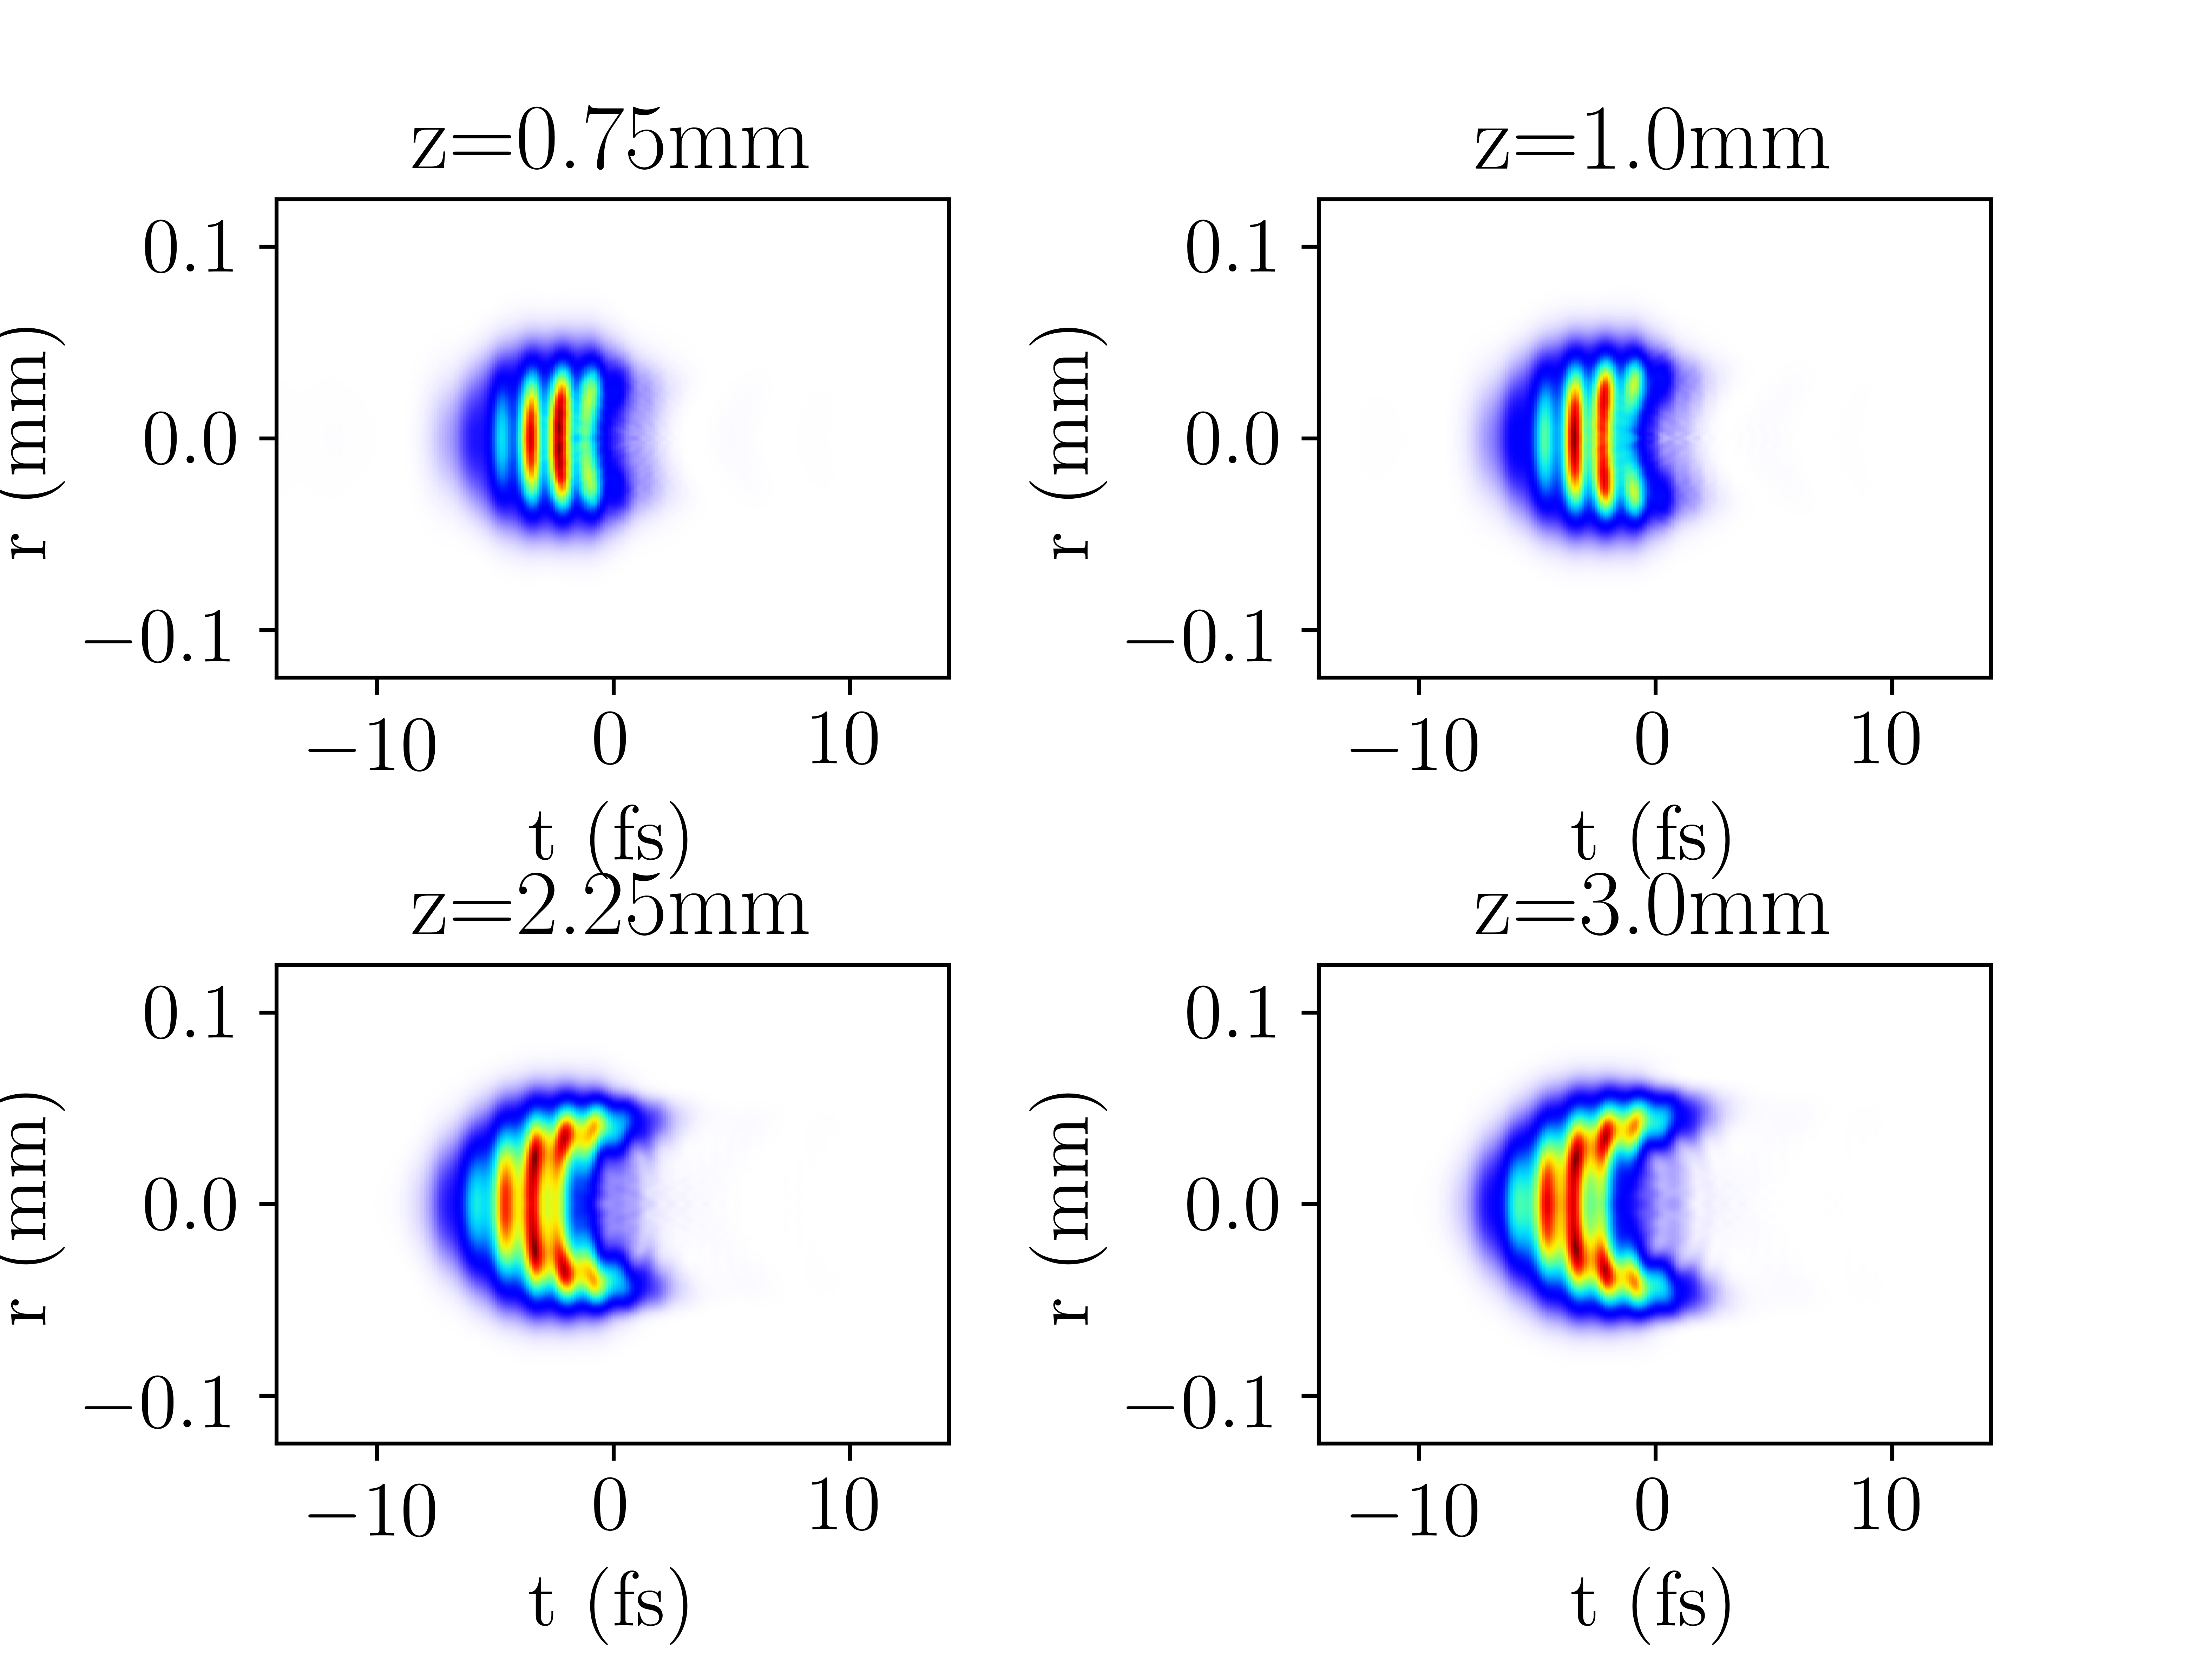
\includegraphics[width=0.5\textwidth]{im/UV_pulse_evolution_Ar_ion}
\caption{Simulated spatiotemporal beam profile of the UV pulses in Argon (150mW NIR power and 0.4bar central pressure). With increasing propagation distance through the 3mm cell leading-edge self-steepening sets in.}\label{im:prop}
\end{figure}
Further investigation reveals that this self-steepening process is  caused by photoionisation effects in the gas, as is seen in Figure \ref{im:profile_Ar}: when turning off ionisation in the simulations no self-steepening in the UV output pulse is observed. This demonstrates that the effects of ionisation are not merely to introduce loss but that it also contributes to pulse shaping. As is shown in Figure \ref{im:profile_Ar}, the ionisation-induced self-steepening has the effect of reducing the UV pulse duration. These results agree with similar studies in the literature, like \cite{reiter2010}. \par 
\begin{figure*}[h]
\centering
 \begin{subfigure}{0.49\textwidth}
        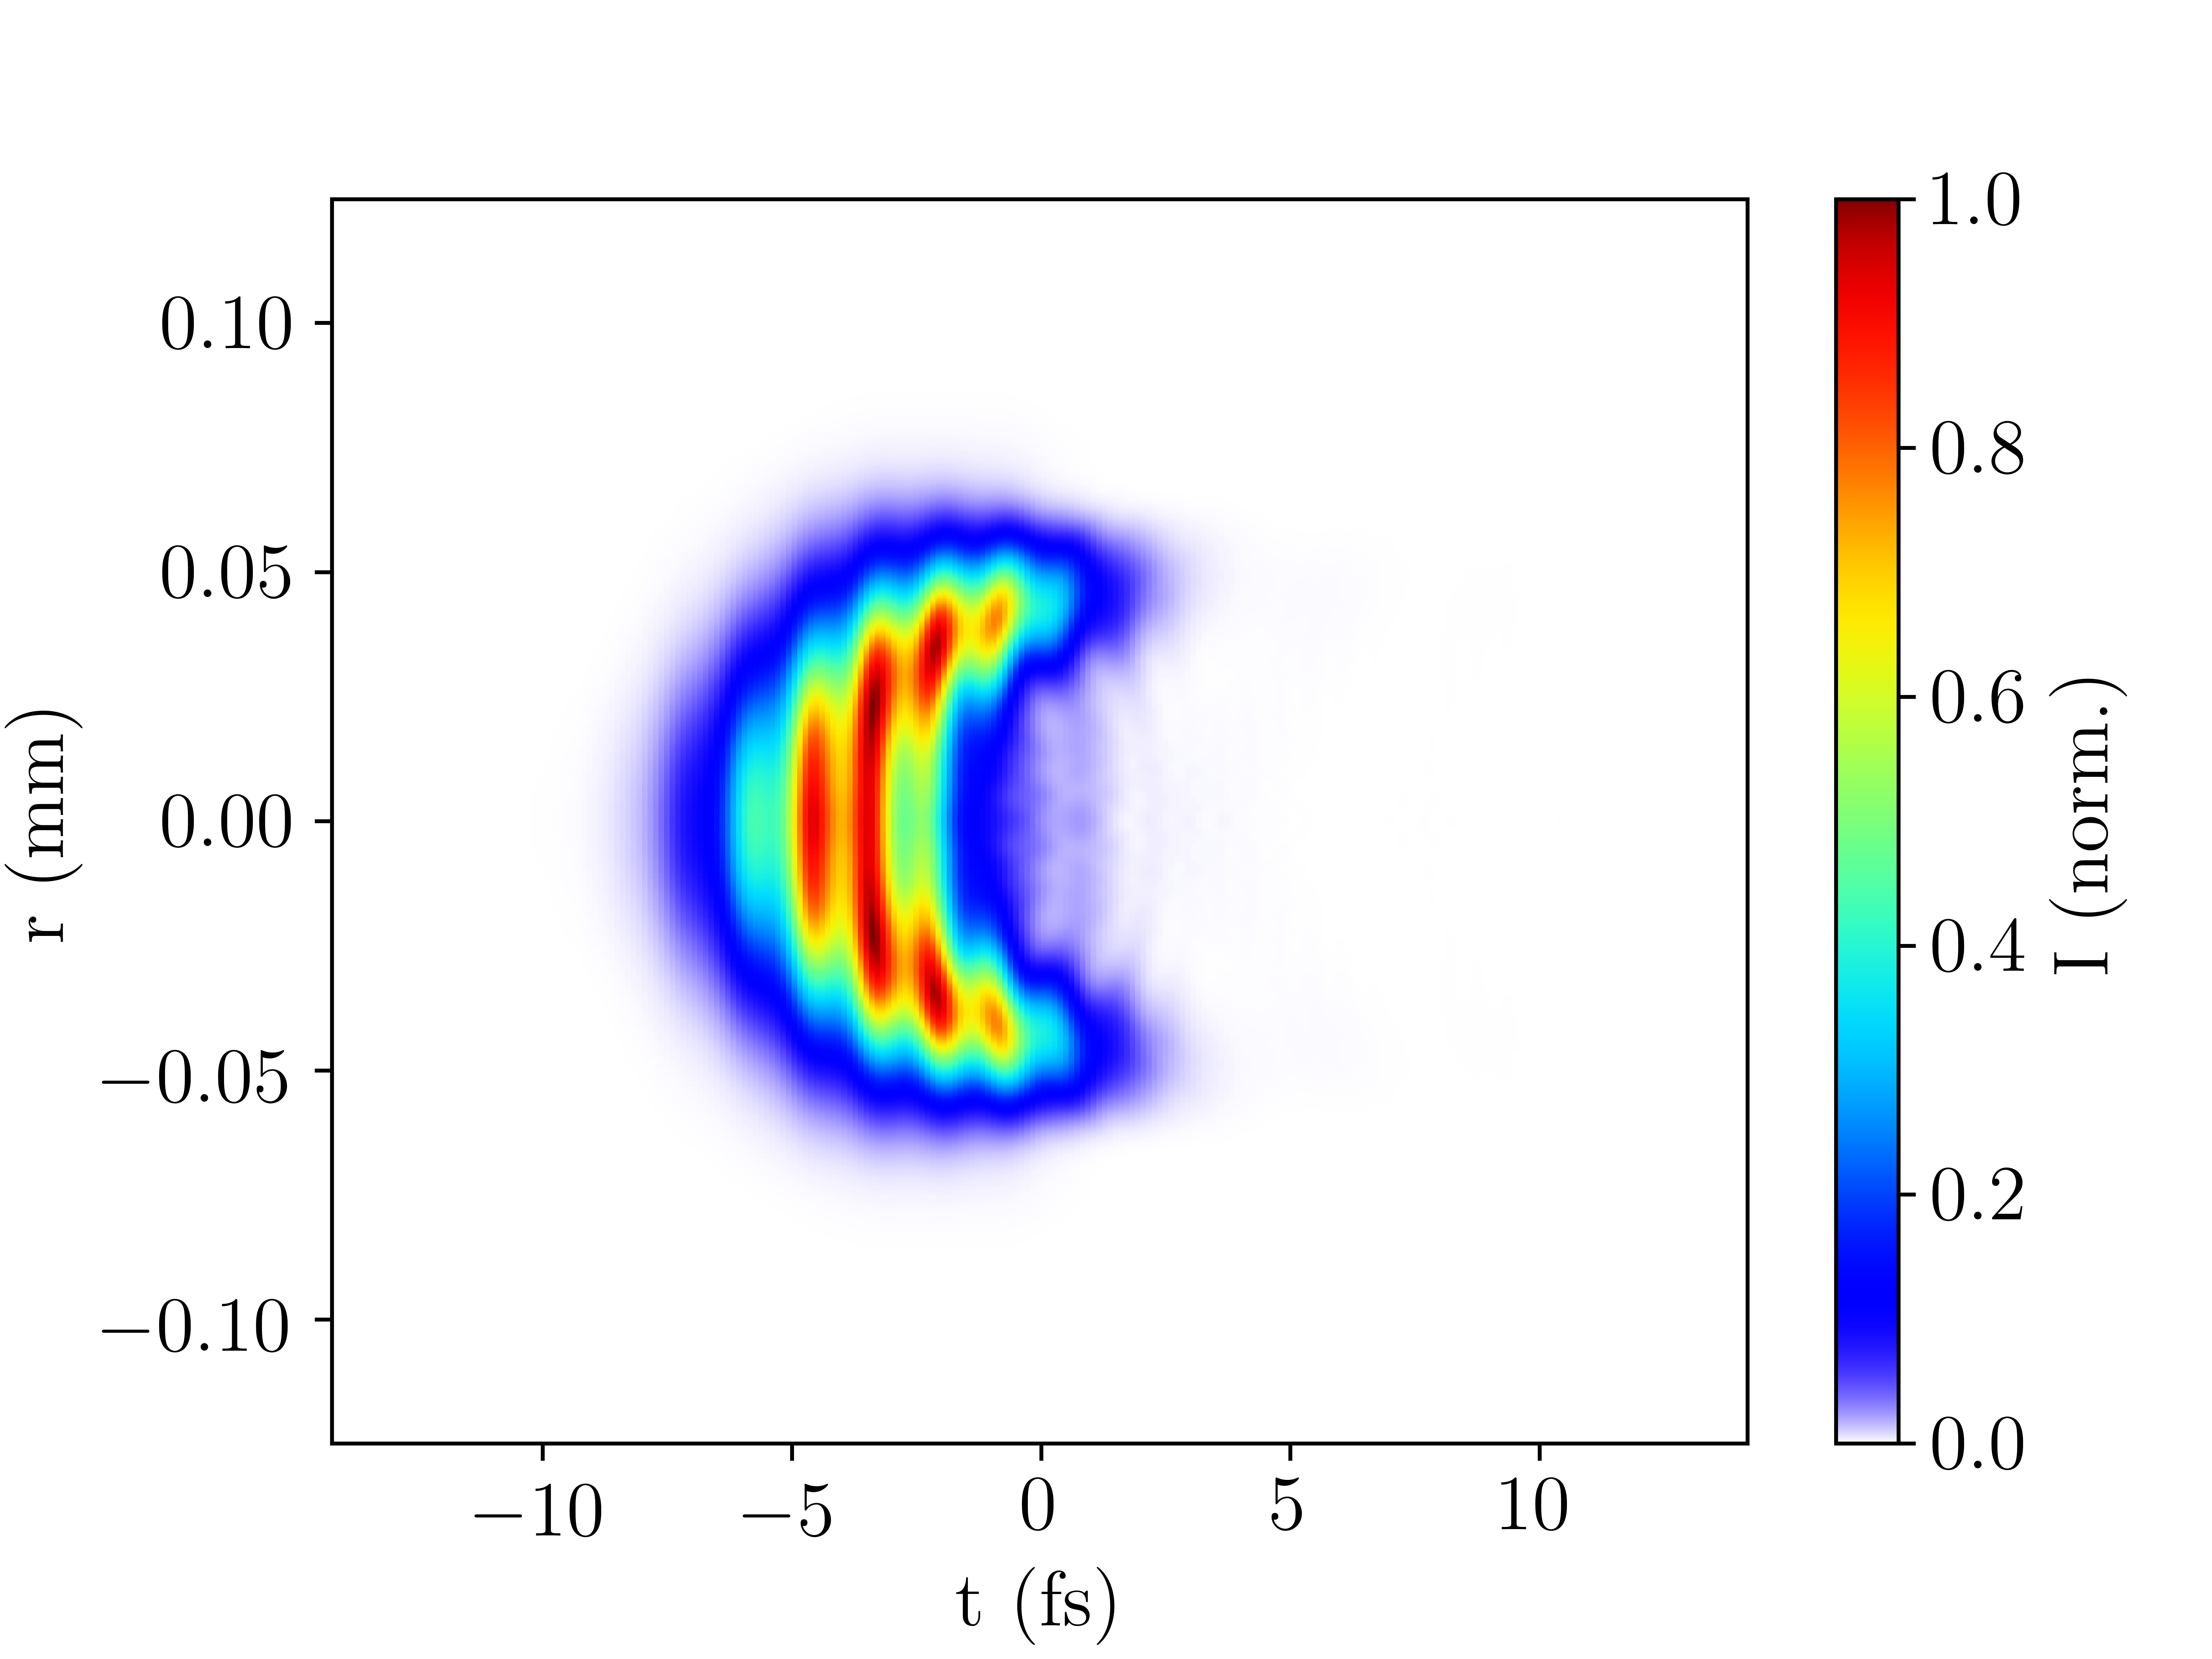
\includegraphics[width=\textwidth]{im/UV_pulse_output_Ar_ion}
    \caption{}
    \end{subfigure}
    \begin{subfigure}{0.49\textwidth}
        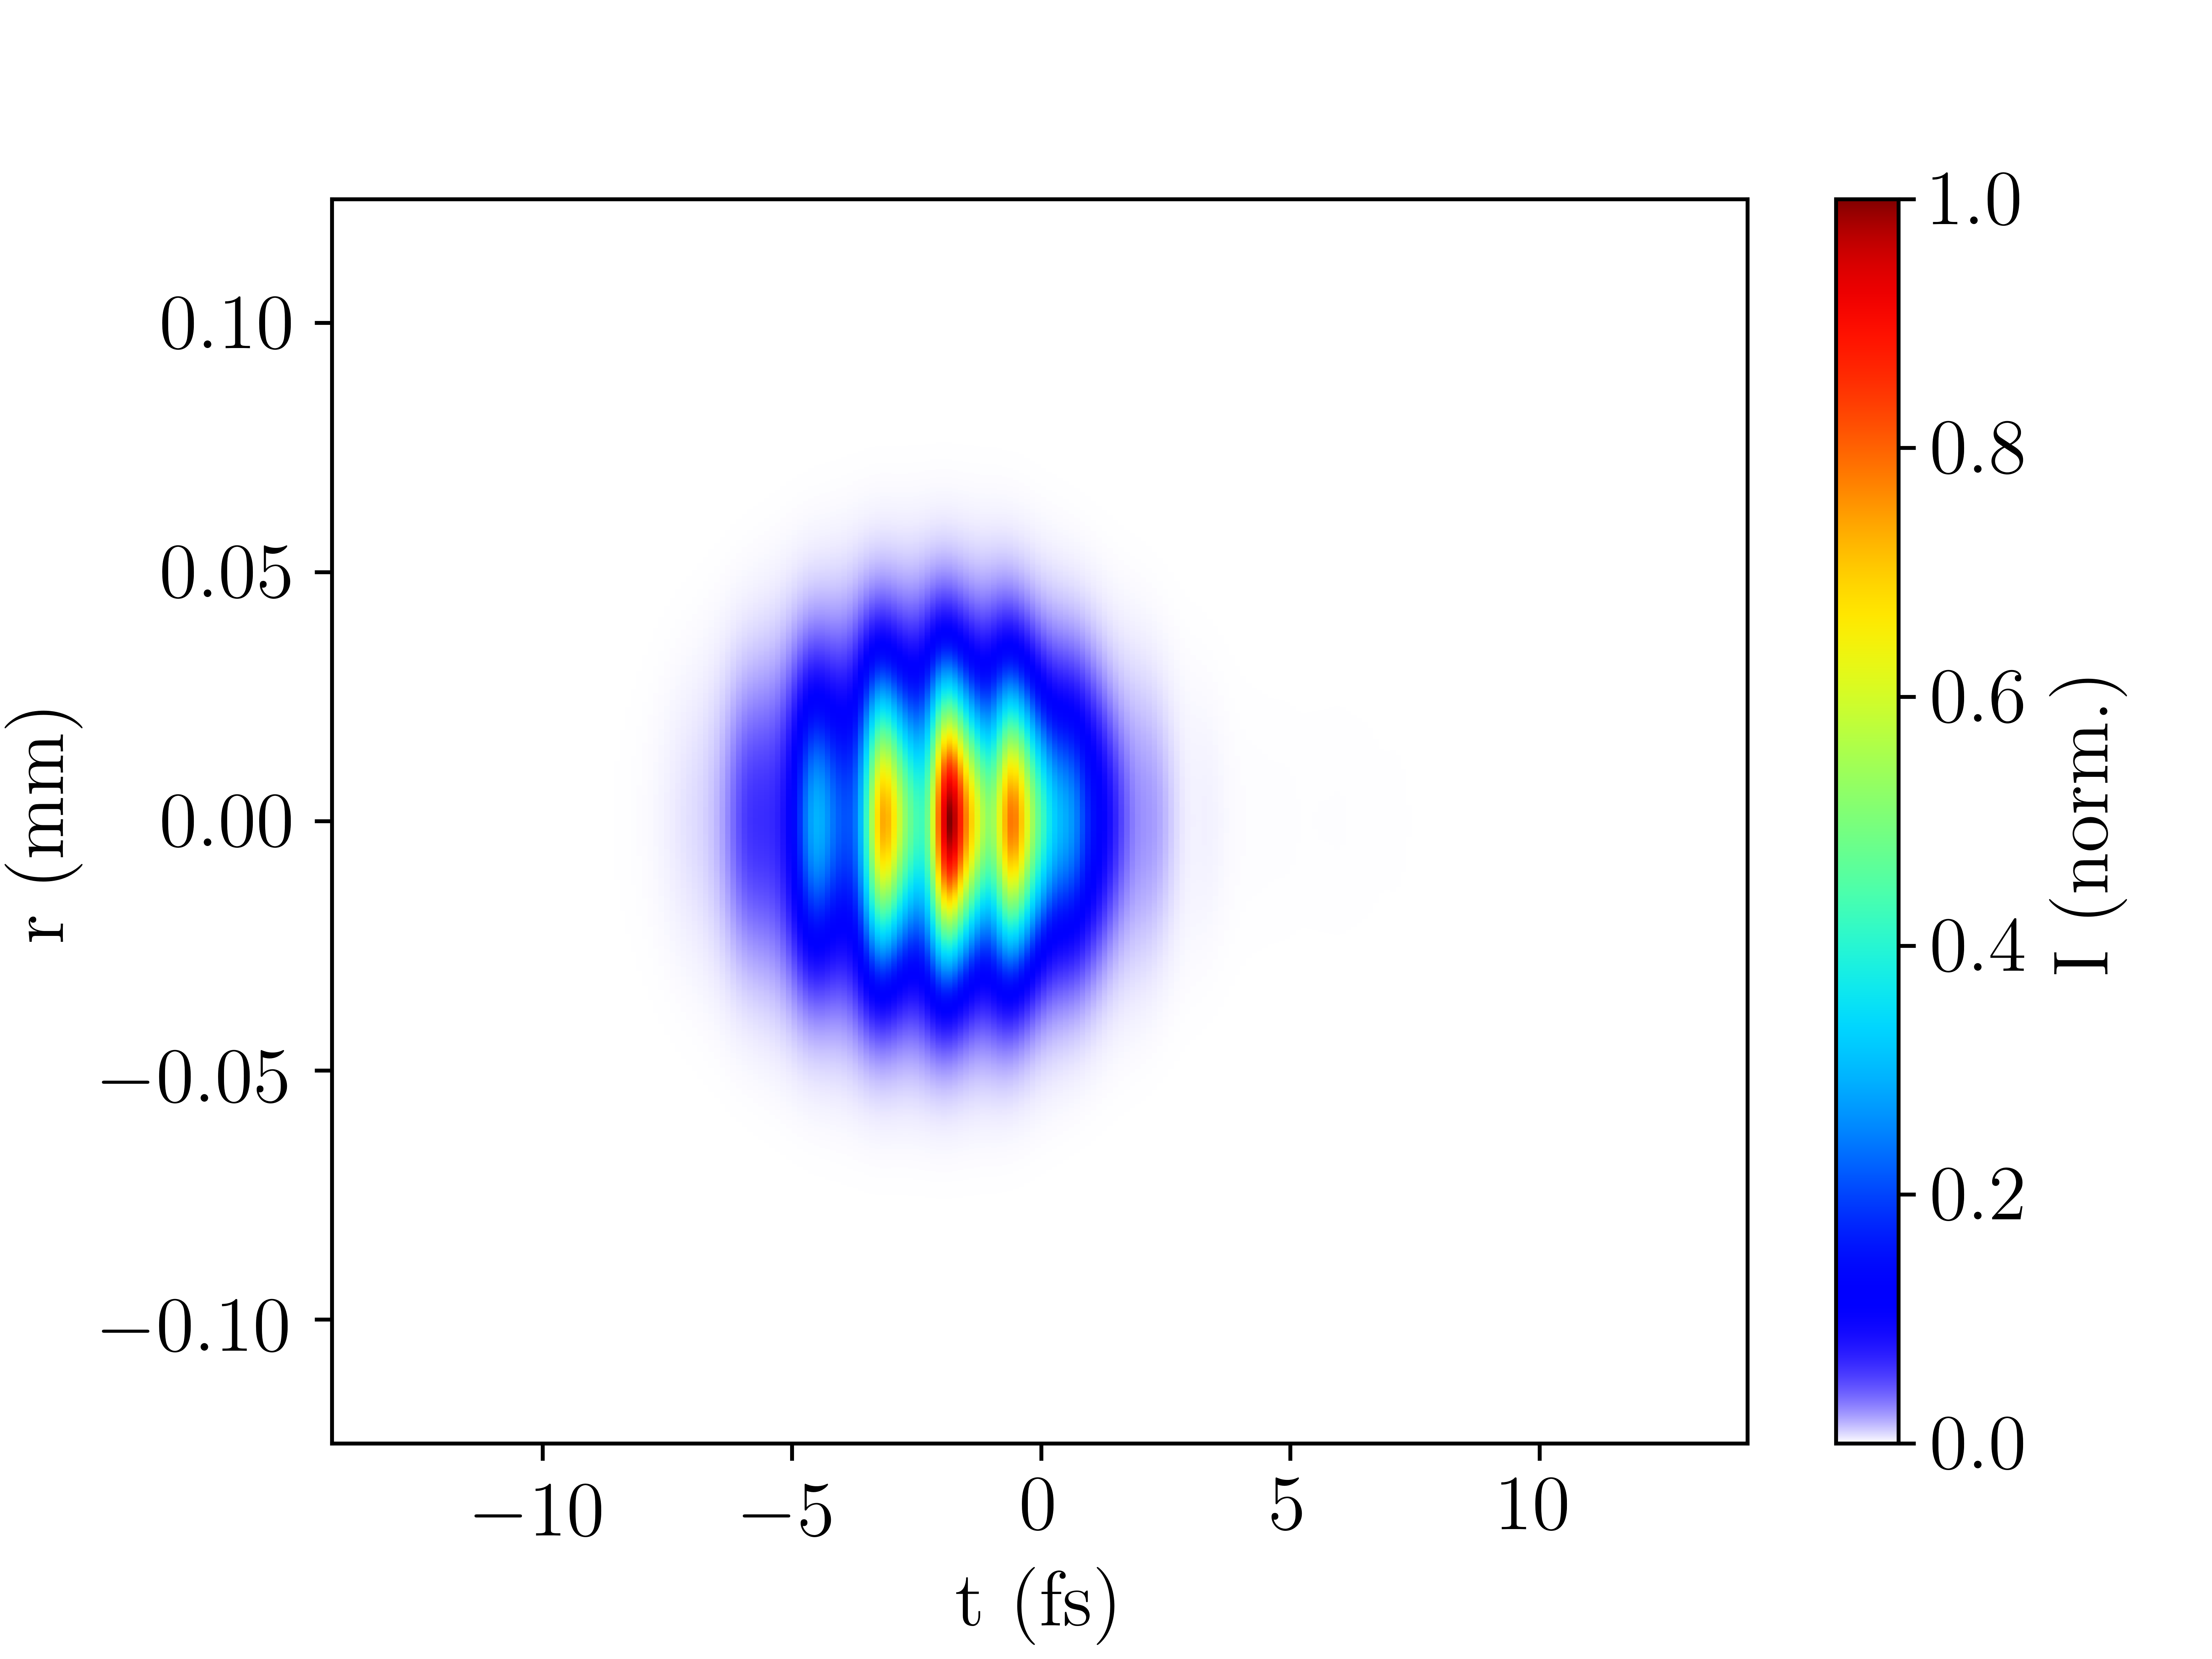
\includegraphics[width=\textwidth]{im/UV_pulse_output_Ar_no_ion}
    \caption{}
    \end{subfigure}   
     \begin{subfigure}{0.49\textwidth}
        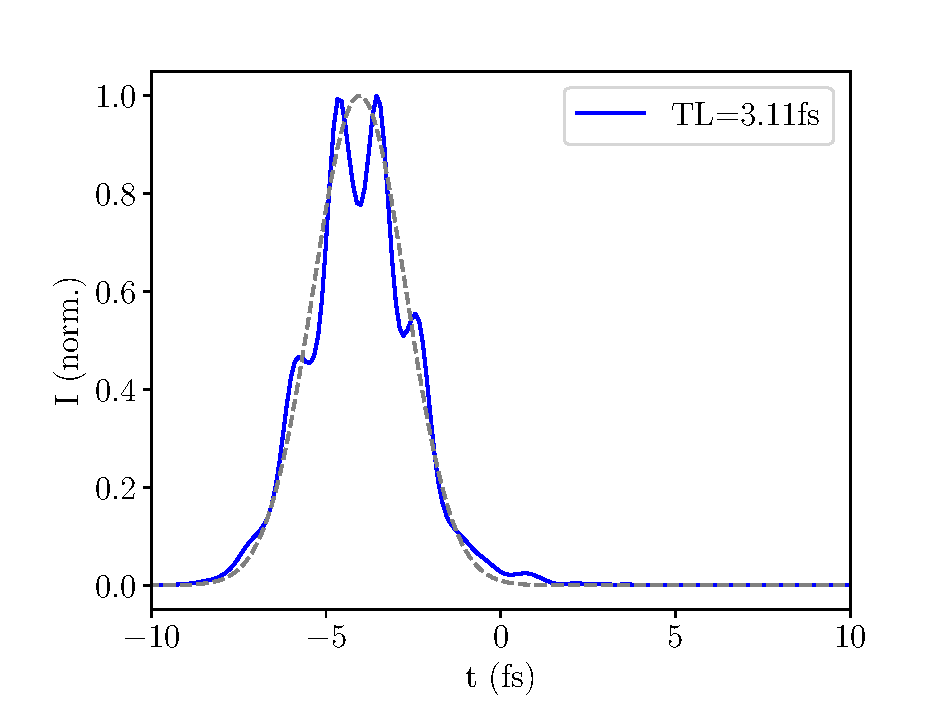
\includegraphics[width=\textwidth]{im/temporal_Ar_ion}
    \caption{}
    \end{subfigure}
    \begin{subfigure}{0.49\textwidth}
        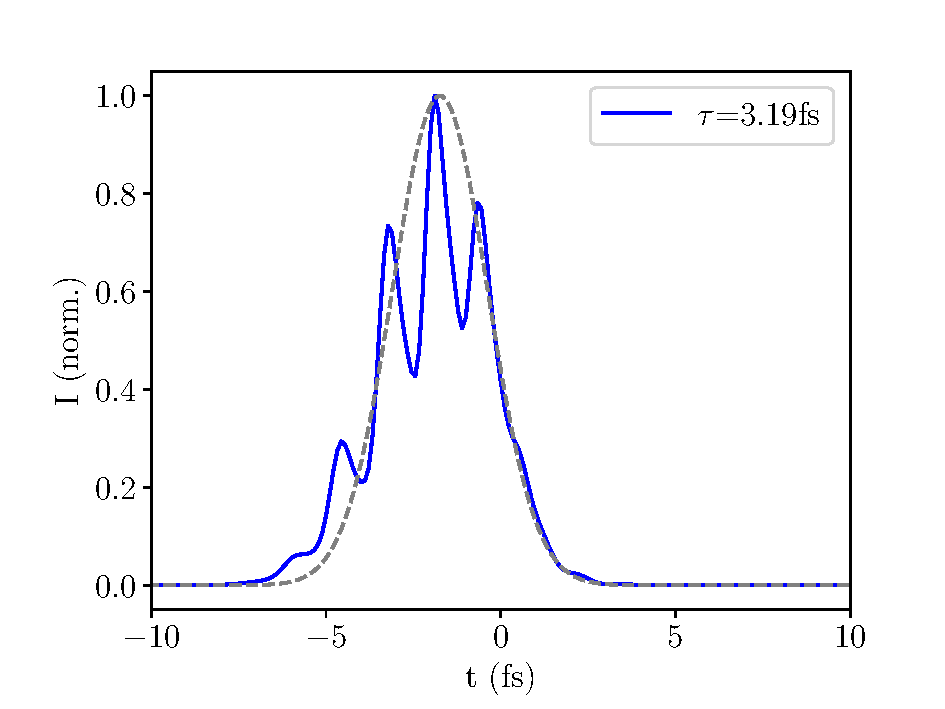
\includegraphics[width=\textwidth]{im/temporal_Ar_no_ion}
    \caption{}
    \end{subfigure}  
\caption{Simulated UV beam profiles at the output using Argon at 150mW NIR power and 0.4bar central pressure. The left column corresponds to simulations including ionisation effects while ionisation is turned off in the right column. }\label{im:profile_Ar}
\end{figure*}
Thus, it has been demonstrated that the simulations, even when limited to the gradient model, can give valuable insights into the process shaping UV generation. 

\subsection{Effects of Chirp}
Another advantage of simulations is that they can be used to probe the effect of changing different experimental parameters. As a case study, this section considers the effect of a chirped NIR input pulse on the generated UV pulses. Figure \ref{im:chirp} shows the effects of both a positively and negatively chirped driving pulse on the UV output spectra. 
\begin{figure*}[h]
\centering
 \begin{subfigure}{0.49\textwidth}
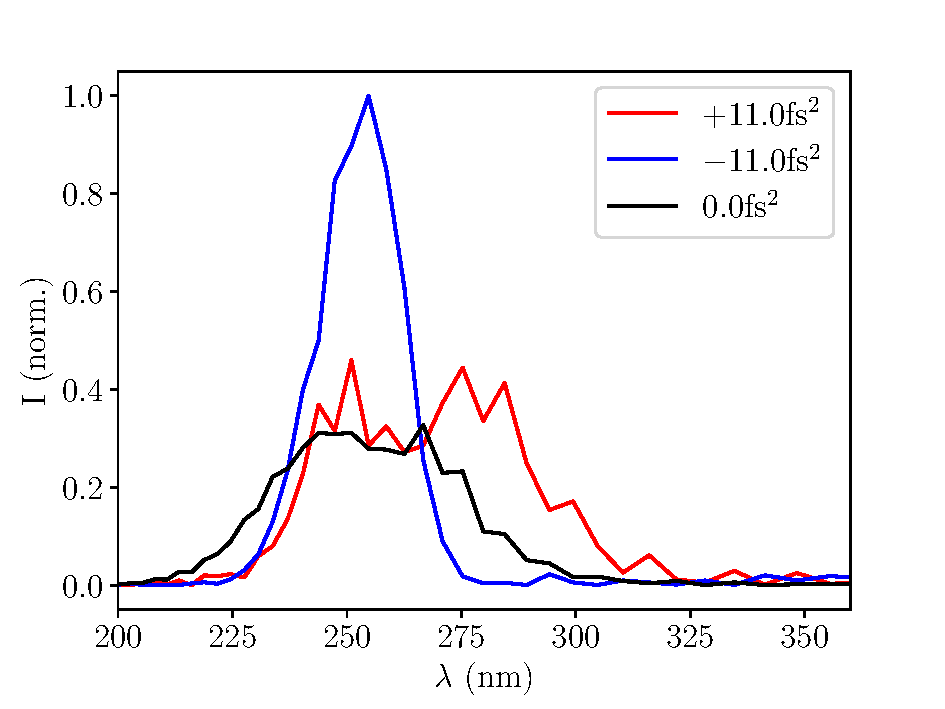
\includegraphics[width=\textwidth]{im/Ar_chirp}
\caption{Argon at 150mW and 0.4bar}\label{im:chirp_Ar}
\end{subfigure}
 \begin{subfigure}{0.49\textwidth}
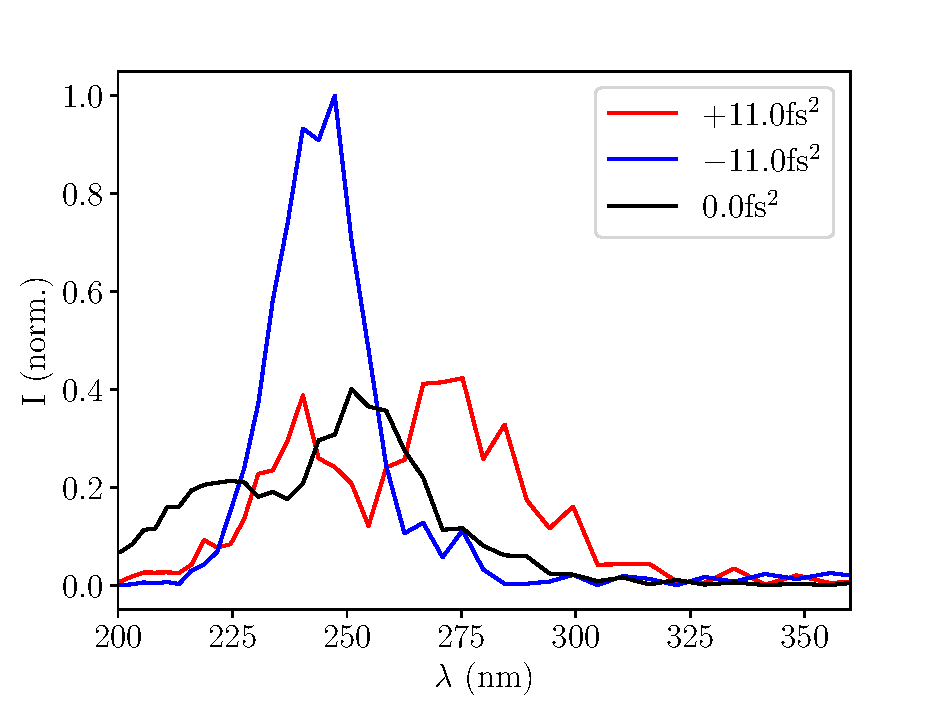
\includegraphics[width=\textwidth]{im/Ne_chirp}
\caption{Neon at 400mW and 2.0bar}\label{im:chirp_Ne}
\end{subfigure}
\begin{subfigure}{0.49\textwidth}
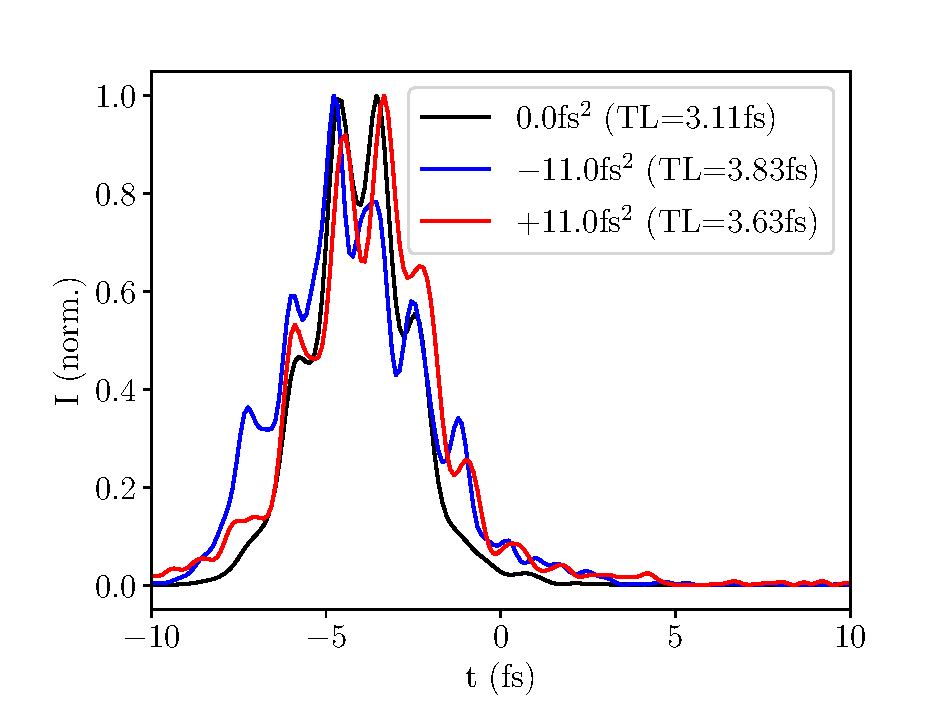
\includegraphics[width=\textwidth]{im/temporal_Ar_chirp}
\caption{Argon at 150mW and 0.4bar}\label{im:chirp_Ar_temp}
\end{subfigure}
\begin{subfigure}{0.49\textwidth}
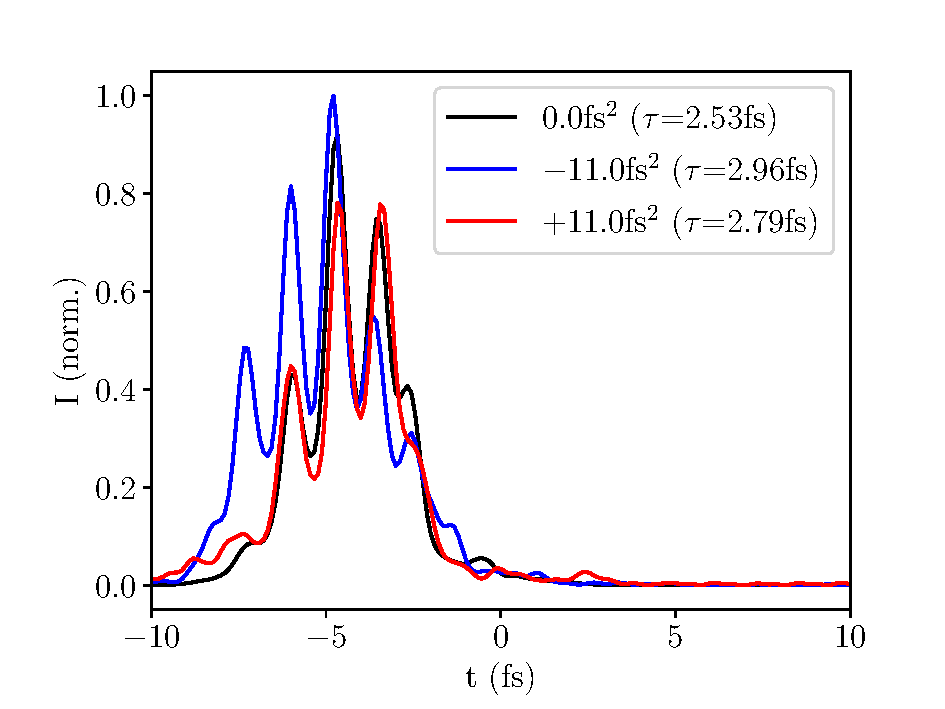
\includegraphics[width=\textwidth]{im/temporal_Ne_chirp}
\caption{Neon at 400mW and 2.0bar}\label{im:chirp_Ne_temp}
\end{subfigure}
\caption{Simulated UV output spectra with different GVD values. The power values in the subfigure captions refer to the NIR beam power and the pressure values to the central cell pressures. Note that the pressures of the simulated spectra have been rescaled.}\label{im:chirp}
\end{figure*}
As can be seen, adding chirp to the input pulse is predicted by the simulations to produce more intense and shorter UV pulses (more details once plots are there!). This prediction can now be tested experimentally. \par 
Thus, it has been demonstrated here how using the simulations one can guide the experimental design by testing the effects of different parameter variations computationally, in a more time-efficient manner. 

\subsection{Comparison of Cells}
As was mentioned earlier, the THG simulations only encompassed the central interaction region and used a simple gradient approximation to model the gas density distribution, due to the lack of appropriate gas flow simulations. The modelling software \textit{COMSOL Multiphysics} was used to obtain some gas density distributions, which do not appropriately capture interactions between the gas molecules, however, and are therefore not suitable for general use. The existing \textit{COMSOL} simulations can nonetheless be used to qualitatively compare the new gas chip to the old cell, which has an identical central interaction region but differs in its pumping system, i.e. in the density distribution outside the THG region. \par 
Figure \ref{im:dens} compares the simulated gas density distributions in the new and the old cell and further to the gradient model in the central interaction region. 
\begin{figure}[h]
\centering
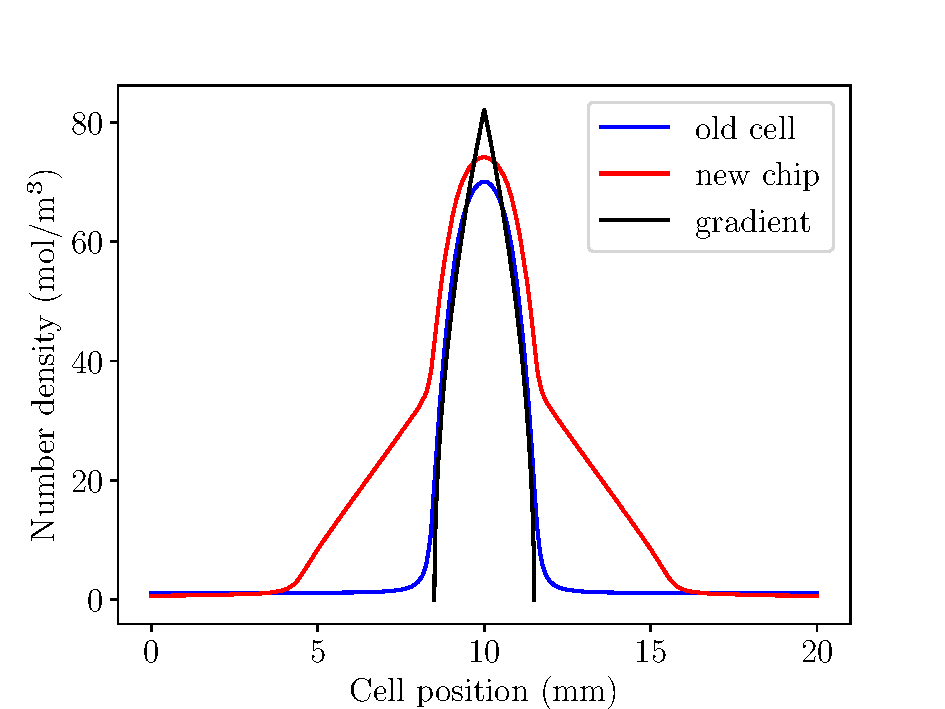
\includegraphics[width=0.5 \textwidth]{im/old_new_comp}
\caption{Comparison of the \textit{COMSOL}-generated gas density distributions of the new and old fused silica chip as well as the gradient model. AT 2 BAR}\label{im:dens}
\end{figure}
Evidently, the gas is less tightly confined in the chips than in the gradient model, i.e. the density at the edges of the central interaction regions drops off more slowly. The main difference between the new and old cells is the density distribution outside the THG region, however: due to the pumping stages in the new chip being closer to the gas inlet, the gas distribution has shorter wings than the old cell. \par 
The UV output spectra obtained with the \textit{COMSOL} models of the new and old cells are shown in Figure \ref{im:coms}. As can be seen, the new chip generates UV pulses that are more intense and have a higher spectral bandwidth than the old cell. This agrees with experimental comparisons of the two designs. \par 
\begin{figure}[h]
\centering
 \begin{subfigure}{0.5\textwidth}
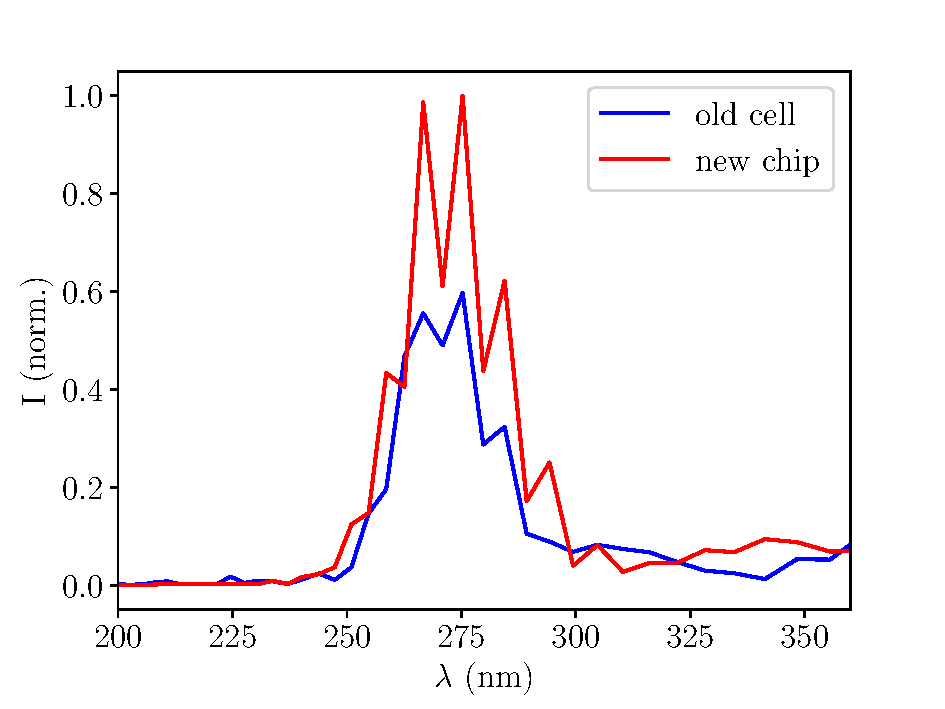
\includegraphics[width=\textwidth]{im/Ar_old_v_new}
\caption{Argon (150mW, 0.4bar)}\label{im:coms_Ar}
\end{subfigure}
 \begin{subfigure}{0.5\textwidth}
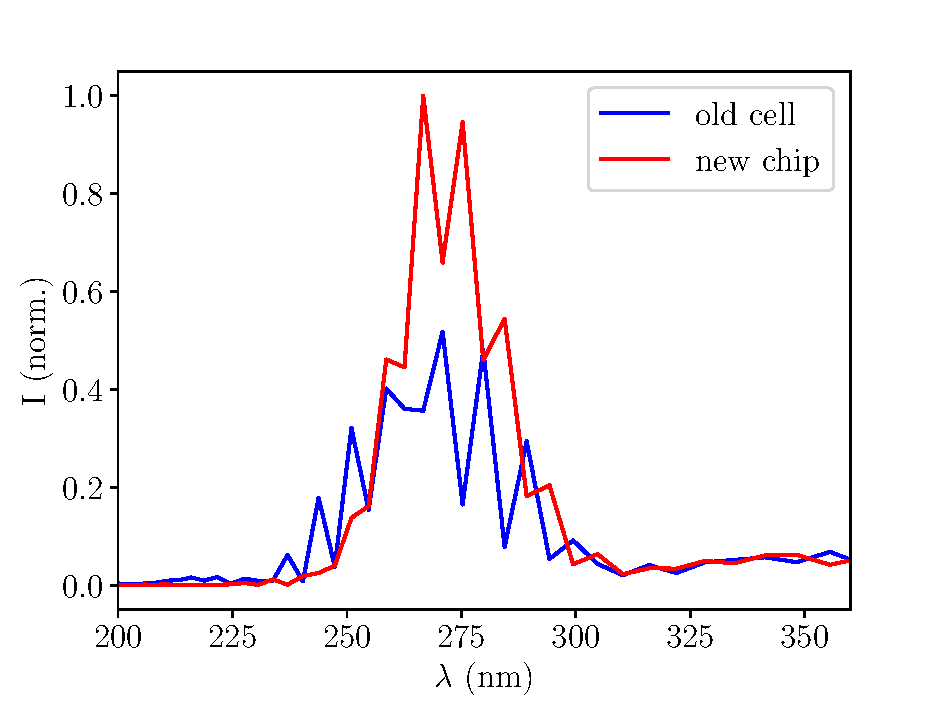
\includegraphics[width=\textwidth]{im/Ne_old_v_new}
\caption{Neon (400mW, 2.0bar)}\label{im:coms_Ne}
\end{subfigure}
\caption{Comparison of the UV output spectra simulated for the new and old gas cells}\label{im:coms}
\end{figure}


\begin{figure}[h]
\centering
 \begin{subfigure}{0.5\textwidth}
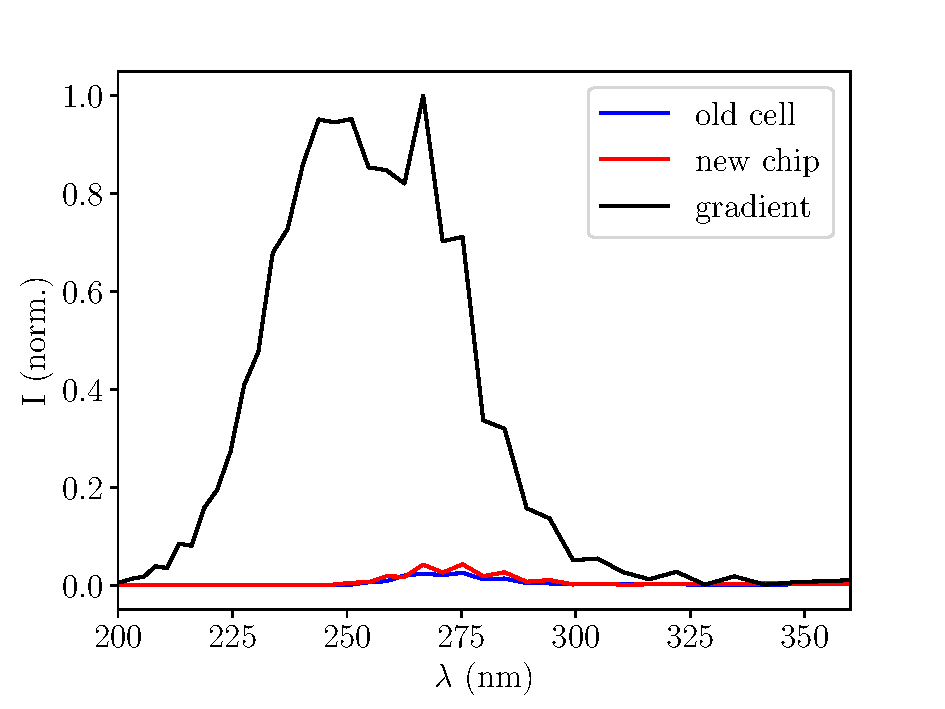
\includegraphics[width=\textwidth]{im/Ar_old_v_new_v_grad}
\caption{Argon (150mW, 0.4bar)}\label{im:coms_Ar}
\end{subfigure}
 \begin{subfigure}{0.5\textwidth}
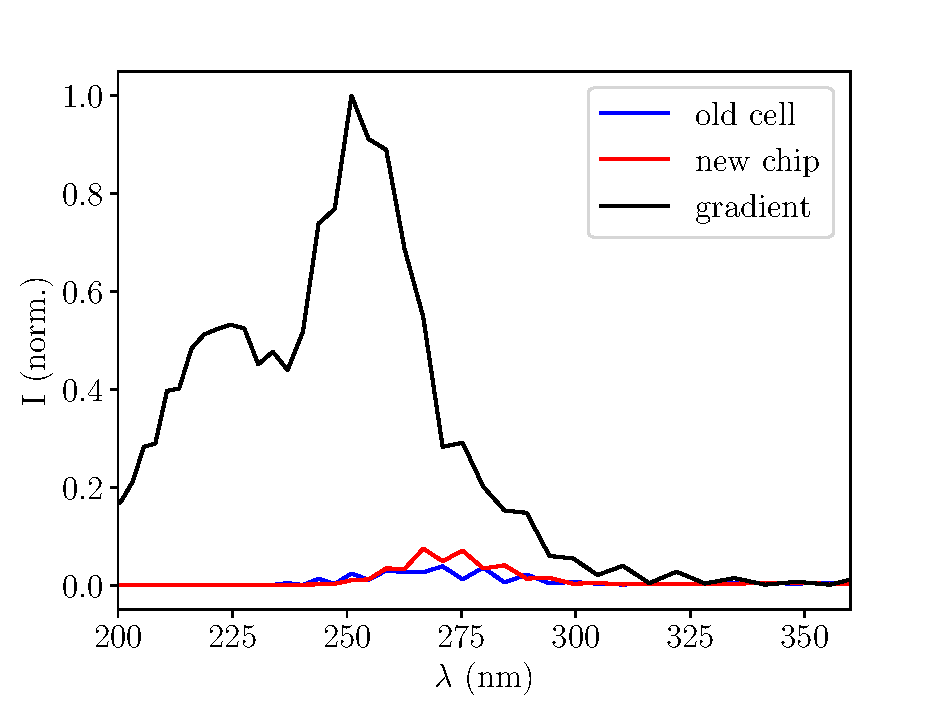
\includegraphics[width=\textwidth]{im/Ne_old_v_new_v_grad}
\caption{Neon (400mW, 2.0bar)}\label{im:coms_Ne}
\end{subfigure}
\caption{Comparison of the UV output spectra simulated for the new and old gas cells}\label{im:coms}
\end{figure}
It is notable how drastically different the simulated spectra produced using the gas density simulations for the new and old chips look to those using the gradient model. This highlights that the UV generation process is highly sensitive to the gas density distribution and confinement. For this reason, the design of the fused silica chip is crucial for production of short yet energetic UV laser pulses. Conceivably, provided that accurate gas flow models are available, the THG simulations could be used to aid in the design of further improved chips. 

\section{Discussion}

The THG simulations produced as part of this project yielded some promising results: qualitative agreement with experimental data and the literature could be observed. Indeed, some of the figures presented in this report will be used in a manuscript submitted to the \textit{Journal of Physics: Photonics}. \par 
There is significant room for further improvement of the simulations. For instance, the measured spatial profile of the NIR input pulses could be fed into the simulations, replacing the Gaussian approximation as well as the assumption of radial symmetry. As the input beam shape and its potential defects, like astigmatisms, have been shown experimentally to affect UV generation it is likely that implementing this degree of freedom in the simulations would have a significant effect. Most importantly, the THG simulations should be extended beyond the 3mm central interaction region in the chip. As the preliminary comparison between the old and new chip in Section 5 showed, the gas density profile outside the central interaction region seems to have a significant effect on UV generation.  A better model of the gas distribution, taking into account nonlinear optical effects as well as absorption outside the central chamber might resolve the misalignment of the simulated and measured energy scales: the preliminary \textit{COMSOL Multiphysics} gas distributions show a change in UV energies compared to considering only the central interaction region of an order of magnitude. Whether the simulated and measured pressure scales can be aligned by an improved gas density model remains to be seen, however, as determining the pressure in the cell is an experimental challenge. \par 
With these improvements, or in their present form, the THG simulations can be used to explore a wide range of experimental parameters that influence UV generation. These include different pressure and beam power regimes, a more thorough investigation of the effects of a chirped input beam, as well as different gases. \par 
Given sufficient future modification and calibration, the THG simulations have the potential to become useful tools in evaluating experimental data as well as theoretically exploring the effects of changing various experimental parameters.  

\section{Conclusion}
This report presented simulations of the nonlinear optical processes used by the CFEL-ATTO group to produce few-femtosecond UV laser pulses. The aim of the simulations was to reproduce the relevant experimental conditions and further to give insights about the parameters and effects shaping the UV generation process. \par 
It has been shown that the simulations could qualitatively reproduce the measured UV spectra and energies to a good degree, despite a misalignment of the pressure and energy scales. The observed discrepancies between simulations and experiment can be attributed to the crude gas density model used at present.  \par 
Further, by considering the spatiotemporal UV beam profile, it was demonstrated that the simulations can give insights into pulse properties that are difficult to access experimentally:the simulations predict ionisation-induced self-steepening to contribute to pulse compression, in agreement with the literature. \par 
Additionally, the simulations indicate that working with chirped driving pulses could further decrease UV pulse durations while increasing UV intensities, which is a robust hypothesis to be tested experimentally. \par 
Finally, using more sophisticated but still incomplete models of the gas density distribution including the pumping stages, the performance of the fused silica chip in which UV generation takes place is compared to a previous design and shown to be more efficient, in agreement with measurements. \par 
Given their success despite the crude gas model used, the simulations presented in this report thus have the potential to become the basis of a robust theoretical framework to complement experiments. 

\section*{Acknowledgments}
I want to thank Josina Hahne for supervising the project and all of her support as well as Vincent Wanie for his additional guidance. I also want to thank Chris Brahms for providing help with \textit{Luna.jl} and the entire CFEL-ATTO group for being so welcoming and friendly. Finally, thank you to Olaf Behnke and Andreas Przystawik for organising the DESY Summer Student programme. 

\section*{References}
\bibliographystyle{osa}
\bibliography{refs.bib}

\end{document}